\documentclass[oneside,11pt,nocover,
  printed, %% This option enables the default options for the
           %% digital version of a document. Replace with `printed`
           %% to enable the default options for the printed version
           %% of a document.
  notable,   %% Causes the coloring of tables. Replace with `notable`
           %% to restore plain tables.
  nolof,     %% Prints the List of Figures. Replace with `nolof` to
           %% hide the List of Figures.
  nolot,     %% Prints the List of Tables. Replace with `nolot` to
           %% hide the List of Tables.
  %% More options are listed in the user guide at
  %% <http://mirrors.ctan.org/macros/latex/contrib/fithesis/guide/mu/fi.pdf>.
]{fithesis3}

%% The following section sets up the locales used in the thesis.
\usepackage[resetfonts]{cmap} %% cmap makes the PDF searchable and copyable
\usepackage[T1]{fontenc}
\usepackage[
  main=english, %% By using `czech` or `slovak` as the main locale
                %% instead of `english`, you can typeset the thesis
                %% in either Czech or Slovak, respectively.
  czech         %% The additional keys allow
]{babel}        %% foreign texts to be typeset as follows:
%%
%%   \begin{otherlanguage}{czech}   ... \end{otherlanguage}

%% The following section sets up the metadata of the thesis.
\thesissetup{
    date          = \the\year/\the\month/\the\day,
    university    = mu,
    faculty       = fi,
    type          = d,
    author        = Petr Velan,
    gender        = m,
    advisor       = {doc. Ing. Pavel Čeleda, Ph.D.},
    title         = {Next Generation Application-Aware Flow Monitoring},
    TeXtitle      = {Next Generation Application-Aware Flow Monitoring},
    keywords      = {network, monitoring, network flow, NetFlow, IPFIX},
    TeXkeywords   = {network, monitoring, network flow, NetFlow, IPFIX},
    bib           = {bibliography.bib,publications.bib,rfcused.bib},
}
\thesislong{abstract}{
    This is the abstract of my thesis, which can

    span multiple paragraphs.

\itodo{
Main contributions:\\
- High-speed flow monitoring (100G, 2x80G)\\
- Addition of application layer information to flow monitoring\\
- Analysis of impact of traffic composition on application flow monitoring\\
- Proposal of new generation of application flow measurement - EventFlow \\

Other contributions\\
- Design of flexible flow collector for application flow processing\\
- Implementation of flexible IPFIX export for flowmon exporter\\
- Survey of methods for encrypted traffic classification\\

TODO: discuss privacy issues (where?)
}
}

\thesislong{thanks}{
    This is the acknowledgement for my thesis, which can

    span multiple paragraphs.
}

\usepackage{makeidx}      %% The `makeidx` package contains
\makeindex                %% helper commands for index typesetting.
%% These additional packages are used within the document:
\usepackage{paralist} %% Compact list environments
\usepackage{amsmath}  %% Mathematics
\usepackage{amsthm}
\usepackage{amsfonts}
\usepackage{url}      %% Hyperlinks
% \usepackage{markdown} %% Lightweight Markup

% TO-DO notes
\usepackage{xargs}
\usepackage[dvipsnames]{xcolor}
\usepackage[colorinlistoftodos,prependcaption,textsize=small,textwidth=35mm]{todonotes}
\newcommandx{\unsure}[2][1=]{\todo[linecolor=red,backgroundcolor=red!25,bordercolor=red,#1]{#2}}
\newcommandx{\change}[2][1=]{\todo[linecolor=blue,backgroundcolor=blue!25,bordercolor=blue,#1]{#2}}
\newcommandx{\info}[2][1=]{\todo[linecolor=OliveGreen,backgroundcolor=OliveGreen!25,bordercolor=OliveGreen,#1]{#2}}
\newcommandx{\improve}[2][1=]{\todo[linecolor=Plum,backgroundcolor=Plum!25,bordercolor=Plum,#1]{#2}}
\newcommandx{\thiswillnotshow}[2][1=]{\todo[disable,#1]{#2}}
\newcommandx{\itodo}[2][1=]{\todo[inline,#1]{#2}}
\newcommandx{\iunsure}[2][1=]{\unsure[inline,#1]{#2}}
\newcommandx{\ichange}[2][1=]{\change[inline,#1]{#2}}
\newcommandx{\iinfo}[2][1=]{\info[inline,#1]{#2}}
\newcommandx{\iimprove}[2][1=]{\improve[inline,#1]{#2}}

% Following fixes use of cline in tables, which is broken by 
% czech babel (- is made into active character)
\makeatletter
\begingroup
\toks0=\expandafter{\@cline{#1}-{#2}\@nil}
\@ifpackageloaded{booktabs}{%
  \toks2=\expandafter{\@@@cmidrule[{#1}-{#2}]{#3}{#4}}%
}{}
\catcode`-=\active
\edef\x{\gdef\unexpanded{\@cline#1-#2\@nil}{\the\toks0}}\x
\@ifpackageloaded{booktabs}{%
  \edef\x{\gdef\unexpanded{\@@@cmidrule[#1-#2]#3#4}{\the\toks2}}\x
}{}
\endgroup
\makeatother

% Definitions style using amsthm package
\newtheoremstyle{defnstyle} % name
    {0em}                        % Space above
    {0em}                        % Space below
    {\itshape}                   % Body font
    {}                           % Indent amount
    {\bfseries}                  % Theorem head font
    {\newline}                   % Punctuation after theorem head
    {.5em}                       % Space after theorem head
    {}  % Theorem head spec (can be left empty, meaning ‘normal’)

\theoremstyle{defnstyle}
\newtheorem{defn}{Definition}[chapter]

% \usepackage{graphicx}
% \usepackage{a4wide}
% \usepackage{tabularx}
% \usepackage{amssymb}
% \usepackage[hyphens]{url}
% \usepackage[titletoc]{appendix}
% \usepackage{color}
% \usepackage{textcomp}
% \usepackage[hidelinks]{hyperref}
% \usepackage{pifont}
% \usepackage[table]{xcolor}
% \usepackage{subfig}
% \usepackage[ruled, lined, linesnumbered,norelsize]{algorithm2e}
\usepackage{multirow}
\usepackage{booktabs}

% Load packages required by fithesis. We can setup those packages after this point
\thesisload

% Quotes in italices with centered reference (package csquotes)
\renewcommand{\mkbegdispquote}[2]{\itshape}
\renewcommand{\mkenddispquote}[2]{\par\centering #1#2}

% Environment for definitions using csquotes for centering
\newenvironment{definition}{\begin{displayquote}\vspace{-1em}\begin{defn}}
{\end{defn}\end{displayquote}}

% Make multiple authors be printed as first et al. (package biblatex)
\ExecuteBibliographyOptions{maxcitenames=2}

\begin{document}

%------------------------------------------------------------------------------
% Include all chapters

\chapter{Introduction}

\itodo{
Motivation for flow monitoring: Rick’s thesis (data retention!) \\
Use introduction from Challenges of Application Flow Monitoring
}

\iimprove{Rewrite, the following is copied from COMSOC article}
A passive network traffic monitoring is an essential tool for network management, analysis, and security. There are several approaches to the passive network traffic monitoring which differ in the amount of reported information. On one hand, router interface counters can be reported using Simple Network Management Protocol to provide basic accounting information. On the other hand, deep packet inspection (DPI) provides detailed information about the content of the traffic and can be used for enforcing security policies or malware detection. The more detailed the analysis is, the more computing power it requires. Flow monitoring is a way of balancing the level of acquired information and necessary resources. Origins of flow monitoring date back to 1991 and the basic idea is to describe each network connection by a single record using the common properties of all packets in such a connection. Detailed information on the history and the current state of flow monitoring can be found in~\cite{Hofstede-2014-Flow}. Due to the level of information aggregation, the flow monitoring can achieve 100\, Gb/s throughput, and is, therefore, suitable for monitoring of large networks of internet service providers (ISP) and data centers.

Flow monitoring support is implemented in practically all enterprise routers and switches. It provides enough information to detect malicious or anomalous behavior and serves as a data source for many network security appliances. However, application-level attacks do not necessarily exhibit anomalous behavior on the network level and may remain undiscovered. As a DPI can discover these attacks more easily, flow monitoring is being enhanced with aspects of the DPI. The resulting method is called application flow monitoring (or measurement). Application flow records contain not only network level data but also information extracted from a payload of packets. Application flow monitoring can be seen as a compromise between the standard flow monitoring and full deep packet inspection: it balances performance and traffic visibility to provide as much information about the traffic as possible while being able to work on high-speed networks. The works of \cite{Cejka-2015-Using} and \citeauthor{Husak-2015-Security}~\cite{Cejka-2015-Using, Husak-2015-Security} are examples of how application flow monitoring can be utilized to discover attacks on application protocol layer.

\section{Network Monitoring}

\itodo{
Little introduction to the network monitoring and especially the flow monitoring.\\
Introduce application flow monitoring as well, so that the reader knows what the RQs are about.
}

\itodo{
Anomaly detection and mitigation at internet scale: a survey\\
\url{http://dl.acm.org/citation.cfm?id=2525023.2525033}\\
\url{http://link.springer.com/chapter/10.1007/978-3-642-38998-6\_7}\\
Popisuje kdo všecko umí měřit flow, ipfix, ...
}

\section{Research Questions \& Approach}

\begin{enumerate}
	\item How can flow measurement benefit from application layer information. [chap 3]
	\item What is the performance impact of adding application layer information to flow monitoring. [chap 4]
	\item How to monitor high-speed networks (100G+), what can be done to accelerate (application) flow monitoring. [chap 4]
	\item Can application layer information be used to derive more information about the traffic (EventFlow). [chap 6]
	\item How can flow monitoring cope with increasing share of encrypted traffic. [chap 5]
\end{enumerate}


\section{Contributions}

\section{Thesis Structure}

\itodo{Network Flow Monitoring - Introduction, explanation of the used terms and concepts. Serves as a thesis background.}

\chapter{Network Flow Monitoring}\label{chap:network-flow-monitoring}

\begin{chapintro}

Flow monitoring is an important part of network accounting and security nowadays. It facilitates large scale intrusion detection and prevention systems, data analysis, capacity planning, data retention, and other operations important for network management. The aim of this chapter is to provide a comprehensive introduction to network flow monitoring. Firstly, the history of flow monitoring is outlined and related technologies are described and compared to flow monitoring. Secondly, the applicability of currently used flow definitions is discussed and an improved definition is proposed, together with a formal notation. The formal notation allows clear description of flow related algorithms and avoids misunderstandings caused by ambiguities of a natural language. To the best of our knowledge, this is the first attempt to formalise the flow creation process that takes into account all input data used in practice. The rest of the chapter presents the flow monitoring process in detail. Issues encountered while deploying and operating flow monitoring infrastructure of CESNET National Research and Education Network are discussed at the end of this chapter. 

With an exception of the novel flow definition, this chapter covers similar topic as the article of \citeauthor{Hofstede-2014-Flow}~\cite{Hofstede-2014-Flow}. The article served as one of the sources of information about history of flow monitoring and as an inspiration for the structure of this chapter. The reader is encouraged to study the article as an additional source of information. It focuses more on the IPFIX protocol and contains extensive information about the capabilities of existing enterprise and open-source software for flow creation and processing. 

%The main contribution of this chapter is the improved flow definition together with its formal notation and formal description of the flow creation process.
The paper related to this chapter is~\cite{Velan-2018-Improving}.

The organisation of this chapter is as follows:
\begin{itemize}
  \item Section~\ref{sec:flow-monitoring-basics} introduces flow monitoring and provides overview of its history and related technologies.
  \item Section~\ref{sec:flow-definition} provides an improved flow definition and based on this definition provides formal description of flow creation process.
  \item Section~\ref{sec:flow-monitoring-architecture} explains flow monitoring architecture.
  \item Section~\ref{sec:flow-monitoring-process} describes the flow monitoring process from packet capture to flow record export.
  \item Section~\ref{sec:flow-data-processing} describes flow data treatment from flow record reception to storage and further processing.
  \item Section~\ref{sec:common-issues} discusses common issues encountered in flow monitoring operation.
  \item Section~\ref{sec:nfm-summary} summarizes the chapter.
\end{itemize}

\end{chapintro}

\newpage

\section{Flow Monitoring Basics}\label{sec:flow-monitoring-basics}

This section describes history and current state of network flow monitoring. We discuss related standards, introduce terminology used throughout this thesis and provide formal definition of a flow. 

\subsection{History of Flow Monitoring}\label{subsec:history-of-flow-monitoring}

The first mention of a flow export can be found in RFC 1272~\cite{rfc1272} published in 1991 by IETF Internet Accounting (IA) Working Group (WG). The goal of the document was to provide background information on Internet accounting. The authors describe methods of metering and reporting network utilization. The RFC defines a metering process as follows:

\begin{displaycquote}{rfc1272}[Internet accounting: Background]
A METER is a process which examines a stream of packets on a communications medium or between a pair of media. The meter records aggregate counts of packets belonging to FLOWs between communicating entities (hosts/processes or aggregations of communicating hosts (domains)).
\end{displaycquote}

The goal at the time was to provide a framework for traffic accounting, however, the common believe at the time was that internet should be free and any form of traffic capture, even for the accounting purposes, is undesirable. This, together with the lack of vendor interest, resulted in the conclusion of the working group in 1993. Note that the negative attitude towards the monitoring returns more than 20 years later~\cite{rfc7258}.

In 1995, \citeauthor{Claffy-1995-Parameterizable} showed a methodology for internet traffic flow profiling based on packet aggregation~\cite{Claffy-1995-Parameterizable}, which started a revival of flow monitoring efforts. The Realtime Traffic Flow  Measurement (RTFM) Working Group was created in 1996 and it had three main objectives. First was to consider current issues relating to traffic measurement, such as security, privacy, policies and requirements on new network protocols. Second was to produce an improved Traffic Flow Model that should provide a wider range of measurable quantities (e.g. IPv6), simpler way to specify flows of interest, better access control  to measured flow data, strong focus on data reduction capabilities and efficient hardware implementation. The third objective was to develop RTFM Architecture and Meter Management Information Base (MIB) as a standards track IETF documents. The effort resulted in 1999 by publishing several RFCs describing new traffic flow measurement framework with an increased flexibility and even a bi-directional flow support~\cite{rfc2722}. Since these documents fulfilled the objectives of the RTFM WG, the group was concluded in 2000. However, no flow export standard was developed as the vendors showed no interest in this area.

Meanwhile, Cisco realized that similar kind of flow information is already stored in a flow cache of their packet switching devices. The purpose of this cache is to speed up packet switching by making a forwarding decision only for the first packet of each flow. Unlike the RTFM flow measurement framework, the primary purpose of flow cache is not accounting nor monitoring, therefore the configuration of measurement process using a flow cache in a switch is severely limited. Despite the limitations, once Cisco introduced its own flow export technology called \Index{NetFlow}, it achieved widespread adoption. The main reason for the extensive adoption was the fact that it was readily available in most Cisco devices with little effort. The NetFlow was patented in 1996 and the first version that became available to general public around 2002 was NetFlow v5~\cite{CiscoSystems-2007-NetFlow}, albeit Cisco newer released any official specification. The NetFlow v5 format simply specified a single set of fields that should be exported from each flow record. Figure~\ref{fig:nf5-fields} shows all fields that were supported by NetFlow v5. Note the lack of support for the IPv6 protocol.

\begin{figure}[t!]
  \begin{center}
    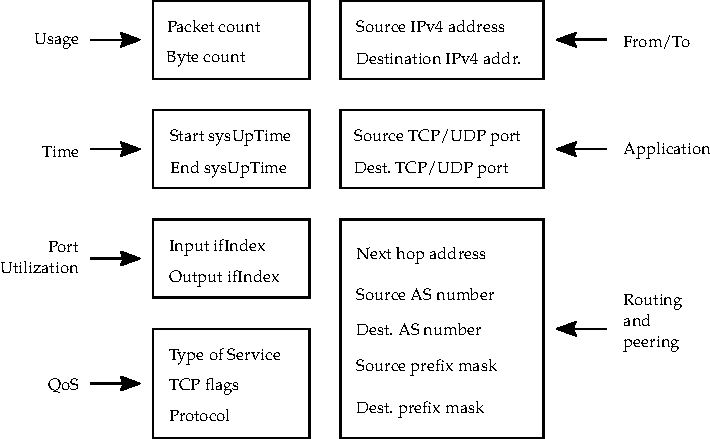
\includegraphics{figures/nf5-fields}
  \end{center}
  \caption{Fields exported by NetFlow v5~\cite{CiscoSystems-2007-NetFlow}.}
  \label{fig:nf5-fields}
% http://www.cisco.com/c/dam/en/us/td/i/000001-100000/60001-65000/60001-61000/60682.ps/_jcr_content/renditions/60682.jpg
\end{figure}

NetFlow v5 was soon obsoleted by NetFlow v9 which remedied some of the deficiencies of the previous version. The state of NetFlow v9 is described in~\cite{rfc3954}. It allowed to define an arbitrary set of fields for export using templates as shown in Figure~\ref{fig:nf9-protocol}. It also introduced support for new protocols, such as IPv6, Virtual Local Area Networks (VLAN), Multiprotocol Label Switching (MPLS), Border Gateway Protocol (BGP) or Multicast. 

\begin{figure}[t!]
  \begin{center}
    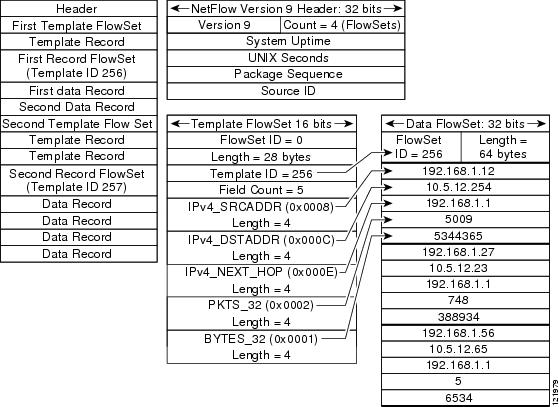
\includegraphics[width=\textwidth]{figures/nf9-protocol}
  \end{center}
  \caption{NetFlow~v9 protocol structure example~\cite{CiscoSystems-2007-NetFlow}.}
  \label{fig:nf9-protocol}
% http://www.cisco.com/c/dam/en/us/td/i/100001-200000/120001-130000/121001-122000/121979.ps/_jcr_content/renditions/121979.jpg
\end{figure}

Other vendors created their own versions of flow exporting protocols, although they retained some level of compatibility with NetFlow. There are JFlow by Juniper, CFlow by Alcatel-Lucent, RFlow by Ericsson, and other protocols. When the potential of flow monitoring for security purposes became realized in 2005~\cite{CiscoSystems-2005-Cisco}, more effort was devoted to extend flow records with information not directly associated with switching. Cisco presented Flexible NetFlow technology~\cite{CiscoSystems-2008-Cisco} in 2006 which allows to dynamically define and export new types of information, such as parts of payloads or traffic identification.

In 2001, it was clear that exporting flow information from switching devices was going to be supported by vendors. However, no standard flow export protocol existed at the time and NetFlow v5 was not yet released to general public. For that reason the IETF started \Index{IP Flow Information Export} (\Index{IPFIX}) WG~\cite{IETF--IP}. The original charter~\cite{IESG-2001-IP} defined six specific goals for the WG: 

\begin{itemize}
    \item Define \emph{``standard IP flow''}.
    \item Devise flow data encoding that support multiple levels of aggregation.
    \item Allow packet sampling in IP flow.
    \item Identify and address security and privacy concerns affecting flow data.
    \item Specify the transport mapping for IP flow information.
    \item Ensure that the flow export system is reliable.
\end{itemize}

The charter was updated over the years to match current requirements. Several vendors were engaged in the IPFIX WG’s activities, most notably Cisco, which significantly contributed from the start. The WG defined set of requirements for the IPFIX protocol~\cite{rfc3917} and evaluated existing candidate protocols~\cite{rfc3955} to decide the most suitable approach in defining the new protocol. The NetFlow v9 specification (RFC 3954) was designed with IPFIX requirements in mind~\cite{Trammell-2011-Introduction} and was released in order to compete in this evaluation (RFC 3955). After the evaluation the NetFlow v9 was chosen as a basis of the new IPFIX protocol. For this reason, IPFIX is sometimes called NetFlow v10 and even starts with protocol version 10 in its header. However, the IPFIX protocol supports many new features and is not completely backwards compatible with NetFlow.

The IPFIX WG did more than just design the IPFIX protocol. In the 29 RFCs published before its conclusion, the WG paid attention to e.g.:
\begin{itemize}
    \item Bidirectional flow export~\cite{rfc5103}
    \item Architecture for IP flow information export~\cite{rfc5470}
    \item Reducing redundancy in flow~\cite{rfc5473}
    \item Definitions of Managed Objects (MIB) for IPFIX~\cite{rfc5815, rfc6615, rfc8038}
    \item IP flow mediation framework~\cite{rfc5982, rfc6183}
    \item IP flow anonymization~\cite{rfc6235}
    \item IPFIX configuration data model~\cite{rfc6728}
\end{itemize}
The IPFIX protocol specification is described by \emph{``Specification of the IP Flow Information Export (IPFIX) Protocol for the Exchange of Flow Information''}~\cite{rfc7011} which became an Internet Standard. The working group was concluded in 2014, however, IPFIX related Internet-Drafts are still being created by involved parties. Further information about IPFIX development is provided by \citeauthor{Brownlee-2011-Flow} in \cite{Brownlee-2011-Flow}.

\subsection{Related Technologies}

Flow monitoring is not the only network monitoring system used to gain information about network behavior. There are other technologies that can be used to monitor network traffic and that can be sometimes confused with flow monitoring. We describe \Index{sFlow}~\cite{Phaal-2004-sFlow}, \Index{IETF Packet Sampling}, \Index{OpenFlow} and Deep Packet Inspection\index{deep packet inspection} in the following text.

sFlow is an industry standard that is supported by number of vendors in their packet switching devices. Its initial specification was published as an Informational RFC~\cite{rfc3176} in 2001, which was the time when packet switching/routing devices with sFlow support became available. The most crucial difference from flow monitoring is that the sFlow does not actually aggregate a stream of packet into a flow record. Instead, it uses sampling to select individual packets and then exports information available about and from these packets. sFlow allows to export data from packet headers, chunks of data from packets and even parse application payloads. It also maintains interface counters and allows their regular export, which is a feature completely unrelated to flow monitoring. sFlow version 5 is the latest version and was published in~\citeyear{Phaal-2004-sFlow}~\cite{Phaal-2004-sFlow}.

In 2002 the IETF started Packet Sampling (PSAMP) Working Group~\cite{IETF--Packet} which was chartered to define a standard set of capabilities for network elements to sample subsets of packets by statistical and other methods~\cite{IESG--Packet}. The result is similar to sFlow, however, the PSAMP uses IPFIX protocol for data export~\cite{rfc5477}. The WG was concluded in 2009 after publishing four RFCs. The proposed standards include sampling and filtering techniques for IP packet selection~\cite{rfc5475}, packet sampling protocol specifications~\cite{rfc5476} and information model for packet sampling export~\cite{rfc5477}.

OpenFlow~\cite{ONF-2012-OpenFlow} is considered to be one of the first Software Defined Networking (SDN) standards~\cite{Singh-2017-Survey, Hu-2014-Survey}. The idea of SDN is to separate control plane and data plane of networking devices. This means that the packet forwarding rules are known only to SDN controllers. The other networking devices that process the traffic ask the controllers what to do with individual flows. After the decision is made for the first packet of the flow, a flow record is kept in the cache so that subsequent lookups do not require the controller interaction. The OpenFlow is a protocol of communication between the networking devices and the controllers. It has been shown by \citeauthor{Yu-2013-FlowSense}~\cite{Yu-2013-FlowSense} that the information stored in the flow caches can be exported using the OpenFlow protocol to the controller and used for network monitoring. Although the approach to network monitoring is somewhat similar to flow monitoring on non-SDN networking devices, there are significant differences. The control traffic itself is utilized to transfer data about new and expired flow records. Therefore, configuration of flow monitoring is directly affected by configuration of SDN network and vice versa. This imposes undesirable restrictions on the flow monitoring process. \citeauthor{Hendriks-2016-Assessing} assess the quality of flow data from OpenFlow devices in~\cite{Hendriks-2016-Assessing}. \citeauthor{Suarez-Varela-2017-Towards} proposes a more scalable solution to mitigate some of the identified problems in~\cite{Suarez-Varela-2017-Towards}. However, the distributed architecture of the monitoring is usually tightly coupled with the deployment of the network controllers. For these reasons, this thesis does not consider SDN specific flow monitoring. It should be noted, that the SDN enabled networking devices can still export valid flow data as defined by the IPFIX standard. In any case, the SDN capabilities are irrelevant for flow monitoring purposes.

Deep Packet Inspection (DPI) is an approach to network data analysis where each packet is dissected up to and including application layer protocol (i.e. packet payload). Although this requires much greater resources than standard flow monitoring, it provides maximum information about network traffic. DPI is an approach, rather than a specific technology, therefore the means of packet capture and information export depend on the particular deployment. For example, sFlow uses DPI to gain information about application layer from packet payloads and exports this information as part of the sFlow protocol. Despite the DPI being diametrically different to flow monitoring, it is being integrated to flow monitoring process to provide the application visibility. This merge balances the detailed view of DPI with the fast and scalable architecture of the flow monitoring. This thesis describes how the DPI is integrated to flow monitoring to create Application Flow Monitoring. Neither sFlow nor OpenFlow are not discussed any further in this work and PSAMP is only mentioned as a packet sampling protocol that can be optionally applied to flow monitoring.


\section{Flow Definition}\label{sec:flow-definition}

To be able to accurately describe the flow monitoring process, we need to have a precise definition of what a flow is. The NetFlow v9 description in~\cite{rfc3954} uses the following definition:

\begin{displaycquote}{rfc3954}[Cisco Systems NetFlow Services Export Version 9]

    An IP Flow, also called a Flow, is defined as a set of IP packets
    passing an Observation Point in the network during a certain time
    interval. All packets that belong to a particular Flow have a set of
    common properties derived from the data contained in the packet and
    from the packet treatment at the Observation Point.

\end{displaycquote}

The Observation Point is defined as a location where IP packets can be observed. The definition says that a flow is a set of packets within a certain time span. Furthermore, the packets in a flow have a set of common properties and these properties are either derived from data contained in the packet data or from packet treatment (e.g. next hop IP address or input interface). Since this definition is quite generic, it covers most of the common IP flow creation techniques.

The IPFIX Protocol is an internet standard~\cite{rfc7011} with its own definition of a flow that builds upon the NetFlow v9 definition. It tries to specify what “properties derived from data contained in packet data” means and differentiates two types of data. The first are the values contained in packet headers, the second type covers the characteristics of the packet itself (e.g. packet length). The definition is as follows:

\begin{displaycquote}{rfc7011}[Specification of the IPFIX Protocol]

    A Flow is defined as a set of IP packets passing an Observation
    Point in the network during a certain time interval.  All packets
    belonging to a particular Flow have a set of common properties.
    Each property is defined as the result of applying a function to
    the values of:

    \begin{enumerate}
    \item one or more packet header fields (e.g., destination IP
        address), transport header fields (e.g., destination port
        number), or application header fields (e.g., RTP header fields
        [5]).

    \item one or more characteristics of the packet itself (e.g., number
        of MPLS labels)

    \item one or more fields derived from packet treatment (e.g., next
        hop IP address, output interface)
    \end{enumerate}
        
    A packet is defined as belonging to a Flow if it completely
    satisfies all the defined properties of the Flow.

\end{displaycquote}

Although this definition is a part of the IPFIX internet standard, there are several problems:
\begin{enumerate}
    \item It is not clear what a \emph{packet header} is. One interpretation is that it includes all protocol headers in the packet up to the packet payload (i.e. application layer). However, the transport header is mentioned explicitly and the example indicates that it can also mean only network layer, in which case the data link layer is completely ignored.
    \item The \emph{characteristics of the packet} are not sufficiently described. One can interpret this as anything that cannot be computed directly from the packet header fields. The example states that a number of certain types of headers are considered as part of the packet's characteristics. The total packet length can be also included here (it was even used as an example in the early drafts in 2002).
    \item The IPFIX standard limits the definition of flows only to IP traffic. 
    However, flows are often created with the use of link layer headers. Moreover, the flow concept works even for non-IP connections, e.g. in technological networks. Therefore, the generic flow definition should allow even non-IP packets. It should be notes that the NetFlow v9 definition of flow explicitly defines IP flows, not generic flows.
    \item Flows using transport header fields cannot be correctly defined for fragmented IP packets, since transport layer information is present only in the first packet fragment. Both NetFlow v9 and IPFIX definitions a set of common properties used to decide which flow the packet belongs to. This must be derived only from the single packet, which is not possible in case of fragmented packets.
\end{enumerate}

In order to provide the most complete definition of flow, we must address all the above mentioned issues. The most direct solution is to start with the NetFlow v9 definition, allow non-IP packets and be clearer about deriving data from previous packets of the same flow which is used for correctly handling the packet fragmentation. Therefore, the definition used in this thesis is as follows:

\begin{definition}\label{def:flow}

    A \emph{\Index{flow}} is defined as a sequence of packets passing an \emph{observation point}
    in the network during a certain time interval. All packets that belong
    to a particular \emph{flow} have a set of common properties derived from
    the data contained in the packet, previous packets of the same \emph{flow},
    and from the packet treatment at the \emph{observation point}.

\end{definition}

There are two more terms connected to flow that need to be defined: \emph{flow key} and \emph{flow record}. The IPFIX definition of the Flow Key needs to be adapted to our definition of flow. We can conveniently shorten the definition to the following:

\begin{definition}\label{def:flow-key}

    A \emph{flow key} is a set of common properties that is used to specify a~\emph{flow}.

\end{definition}

A flow record is basically a tuple containing the flow key and other properties measured for the flow. Moreover, we allow inclusion of more information about the flow that is derived from external sources. An example can be a name of a user to which particular IP address belonged at the time of measurement. The following definition reflects that:

\begin{definition}\label{def:flow-record}

    A~\emph{\Index{flow record}} is a tuple which describes a particular \emph{flow} containing values of:

    \begin{enumerate}
        \item the \emph{flow key} used to specify the \emph{flow},
        \item other properties of the \emph{flow} derived from:
        \begin{enumerate}
            \item data contained in the packets of the \emph{flow},
            \item the packet treatment of the \emph{flow} at the \emph{observation point},
            \item external source of information.
        \end{enumerate}
    \end{enumerate}

\end{definition}

To make the definitions above clearer, we provide an example of concrete properties that might be contained in a flow record in Table~\ref{tab:flow.properties}. The table shows examples of flow record properties that can be derived from packet data and packet treatment. The properties can be aggregated when the derived value differs between individual packets of the flow or where counters such as the number of packets are involved. A~summation function is usually applied to the number of bytes in each packet, TCP flags are aggregated using a logical OR function, the flow start timestamp is derived using a minimum function on each packet timestamp. The non-aggregated properties may be used as part of a flow key.

The definition of flow record states that each flow record describes a particular flow. Moreover, in the rest of this thesis, we make the assumption that each flow is described by a single flow record. This is particularly important for long-lived flows that are terminated by an active timeout. Either the whole flow can be terminated and a new one started, or the flow can continue and only the matching flow record can be expired. Multiple flow records are created in the latter case. We use the former interpretation since it allows to simplify the following definitions.

\begin{table}[ht!]
    \centering
    \begin{tabular}{lll}
    \toprule
                                               & \textbf{Aggregated properties}  & \textbf{Non-aggregated properties}  \\ \midrule
    \multirow{3}{*}{\textbf{Packet data}}      & Number of bytes                 & Source IP address                   \\ 
                                               & TCP flags                       & Destination port                    \\ 
                                               & Time to Live                    & Transport protocol                  \\ \midrule
    \multirow{2}{*}{\textbf{Packet treatment}} & Number of packets               & Input interface number              \\ 
                                               & Flow start timestamp            & Next-Hop IP address                 \\ \bottomrule
    \end{tabular}
    \caption{Examples of Flow Properties}
    \label{tab:flow.properties}
\end{table}

Definition~\ref{def:flow} states what the flow is. Although we tried to be as explicit as possible, the definition is informal and therefore subject to different interpretations. For this reason we now provide a formal definition of flow, which not only refines the informal definition, but also provides a guide to the construction of the flows.

\begin{defn}
Let $P$ be a set of all packets. Let $T$ be a set of packet treatment information. We define a set of \Index{extended packets}
\begin{equation*}
    \widehat{P} = P\times T,
\end{equation*}
so that $\widehat{p} \in \widehat{P}$ denotes a packet $p$ together with its packet treatment information. Let $\mathbb{S}$ be a set of indexes of packets observed at an \emph{observation point}:
\begin{equation*}
    \mathbb{S} = \{1, \ldots, n\} \lor \mathbb{N},
\end{equation*}
where $n \in \mathbb{N}$ is the number of observed packets when the number is finite.

We denote sequence of packets and extended packets observed at an \emph{observation point} respectively:
\begin{align*}
    \mathcal{P} &= (p_i)_{i \in \mathbb{S}},\, p_i \in P,\\
    \widehat{\mathcal{P}} &= (\widehat{p}_i)_{i \in \mathbb{S}},\, \widehat{p}_i \in \widehat{P}.
\end{align*}
\end{defn}
Both sequences are of size $|\mathbb{S}|$. 

Let us now define a \emph{\Index{flow selection function}} $\varphi$ which takes a sequence of extended packets and a new extended packet and decides whether they form a flow. We will use this function to determine whether a newly observed packet belongs to an existing flow.
\begin{defn}\label{def:flow-selection-function}
Let $\widehat{P}^*$ be a set of all finite sequences of extended packets, $\widehat{P}$ be a set of extended packets. We say that a function of type
\begin{equation*}
    \varphi: \widehat{P}^*\times \widehat{P} \to \{true,false\}
\end{equation*}
is a \emph{flow selection function}.
\end{defn}

Before we give a formal definition of a flow\index{flow!formal definition of}, we provide the following intuition for our definition. A flow $\mathcal{F}$ is a sequence of packets defined by a sequence of extended packets with indexes in $\mathbb{S}$ and a \emph{flow selection function} $\varphi$. We require that a packet belongs to a flow if it is determined by all previous packets of that flow. Therefore we construct the flow by induction as described in Algorithm~\ref{alg:flow-construction}.

\begin{algorithm}
    \caption{Construction of a flow}
    \label{alg:flow-construction}
    \begin{algorithmic}[1]
        \STATE Denote $\mathbb{I}$ the set of packet indexes that belong to the flow $\mathcal{F}$
        \STATE Start with $\mathbb{I} = \emptyset$
        \WHILE{An index $k$ of the first extended packet $\widehat{p}_k$ for which $\varphi((\widehat{p}_n)_{n\in \mathbb{I}},\, \widehat{p}_k) = true$ exists}
            \STATE Add $k$ to $\mathbb{I}$
        \ENDWHILE
        \STATE The flow $\mathcal{F}$ is a sequence of packets with indexes from $\mathbb{I}$
    \end{algorithmic}
\end{algorithm}

We shall now define set $\mathbb{I}$ of indexes from $(\widehat{p}_i)$ selected using \emph{flow selection function} $\varphi$, and flow $\mathcal{F}$ so that it conforms with the Definition~\ref{def:flow} as follows:
\begin{defn}\label{def:formal-flow}
Let $(p_i)_{i \in S}, (\widehat{p}_i)_{i \in S}, S \subseteq \mathbb{S}$ be (possibly finite) mutually corresponding sequences of packets and extended packets respectively, $\varphi$ a \emph{flow selection function}.

We define a \emph{flow index set} $\mathbb{I} = \mathbb{I}\left((\widehat{p}_i)_{i \in S},\, \varphi\right)$ as 
\begin{align*}
\mathbb{I} &= \lim_{i \to \infty} J_i \text{, where } J_i \text{ is defined inductively over }i \in \mathbb{N} \text{ as:} \notag\\
J_i &= \left\{
    \begin{array}{ll}
        \left\{\min\left\{ \alpha \in S \mid \varphi(\widehat{p}_{\alpha}) = true \right\}\right\} & \text{for } i = 1 , \\[0.7em]
        J_{i-1} \cup \{\min\{ \alpha \in S \mid \alpha > \sup(J_{i-1}), & \multirow{2}{*}{\text{for } $i > 1$.} \\
        \quad \varphi((\widehat{p}_n)_{n\in J_{i-1}},\, \widehat{p}_{\alpha}) = true \}\} &
    \end{array}\right.
\end{align*}

Finally, we define flow $\mathcal{F} = \mathcal{F}\left((p_i)_{i \in S},\, \mathbb{I}\right)$ as:
\begin{equation*}
    \mathcal{F} = (p_i)_{i \in \mathbb{I}},\, p_i \in \mathcal{P}.
\end{equation*}

\end{defn}

Since we need the $\min$ function to be defined for an empty set (the cases where no flow is defined and where we have already added all possible indexes from $\mathbb{S}$), we define
\begin{equation*}
    \left\{\min\ \emptyset \right\} = \emptyset
\end{equation*}

Definition~\ref{def:formal-flow} of flow creates a single flow for a sequence of extended packets $\widehat{\mathcal{P}}$ and a \emph{flow selection function} $\varphi$. The flow $\mathcal{F}$ is selected based on the first extended packet accepted by $\varphi$. Since we naturally expect that every packet is a part of only a single flow, we can construct a sequence of flows $(\mathcal{F}_i)_{i \in \mathbb{N}}$ by induction as described in Algorithm~\ref{alg:flow-sequence-construction}.

\begin{algorithm}
    \caption{Construction of a sequence of flows}
    \label{alg:flow-sequence-construction}
    \begin{algorithmic}[1]
        \STATE Denote $S_1 = \mathbb{S}$
        \STATE Set counter $i = 1$
        \REPEAT
            \STATE Apply the \emph{flow selection function} $\varphi$ to extended packets with indexes in $S_i$
            \STATE Denote indexes of matching extended packets $\mathbb{I}_i$
            \STATE Flow $\mathcal{F}_i $ is a sequence of packets with indexes from $\mathbb{I}_i$
            \STATE Remove indexes in $\mathbb{I}_i$ from $S_i$, denote the new sequence $S_{i+1}$
            \STATE Increment counter $i = i + 1$
        \UNTIL{$\mathcal{S}_i$ is empty}
    \end{algorithmic}
\end{algorithm}

Let us now provide a more formal definition of a sequence of flows $(\mathcal{F}_i)_{i \in \mathbb{N}}$.
\begin{defn}\label{def:formal-flow-sequence}
Let $\mathcal{P}, \widehat{\mathcal{P}}$ be sequences of packets and extended packets respectively, $\varphi$ a \emph{flow selection function}. We define the sequence $(\mathcal{F}_i)_{i \in \mathbb{N}}$ of flows inductively:
\begin{align*}
    \mathcal{F}_i &= \mathcal{F}_i\left((p_j)_{j\in S_i},\, \mathbb{I}_i\right) \text{, where} \\
    S_1 &= \mathbb{S}, \\
    S_i &= S_{i-1} \setminus \mathbb{I}_{i-1}, \\
    \mathbb{I}_{i} &= \mathbb{I}_i\left((\widehat{p}_j)_{j \in S_i},\, \varphi\right).
\end{align*}
\end{defn}

Definition~\ref{def:formal-flow-sequence} provides a guide to constructing a sequence of flow records. The procedure can be easily modified to run in real time so that each newly observed extended packet can be added to the appropriate flow. In our definition, we want every packet to be a part of only a single flow. Therefore, we apply the \emph{flow selection function} $\varphi$ to each pair of existing flow (enriched by packet treatment information) and the new extended packet. Then, we add the packet to the first flow that matches. If none of the existing flows match, we apply the function $\varphi$ to this packet only and start a new flow if necessary. 

From this, we can see that the flow creation process depends solely upon the implementation of the \emph{flow selection function}. We will shortly discuss common implementations in the Subsection~\ref{subsec:flow-creation}.

The condition for every packet to be part of exactly one flow might be too constricting in some cases. It is possible to remove the condition and simply start building each flow from a next extended packet in the sequence. However, this will create many overlapping flows that contain mostly the same packets but start with a different one. This problem would need to be addressed should such a definition be used.

\section{Flow Monitoring Architecture}\label{sec:flow-monitoring-architecture}

Deployment of flow monitoring on a network requires several steps: Capturing packets at one or more observation points, assigning packets to flows, creating and exporting flow records for the flows, and finally collecting, storing, and processing of the exported flow records. 
The Figure~\ref{fig:flow-monitoring-process} shows a high level overview of the whole process. Flow monitoring process encompasses packet capture, flow creation, and creation and export of flow records. Flow data processing comprises of flow record collection, storage, and further processing. Note that the flow records can be processes directly without storing. This approach is called \emph{stream processing}. It is also possible to manipulate the flow records in transition between the export and collection. The IPFIX working group specified a framework called IP Flow Information Export Mediation~\cite{rfc6183} which describes this process. However, description of this process is outside the scope of this thesis.

\begin{figure}[t!]
  \begin{center}
    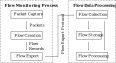
\includegraphics{figures/flow-monitoring-process}
  \end{center}
  \caption{High Level Flow Monitoring Schema}
  \label{fig:flow-monitoring-process}
\end{figure}

This rest of section explains basic terminology and components of the flow monitoring architecture and describes the most commonly deployed flow monitoring architectures.

\subsection{Terminology}

The IPFIX working group published several documents where the architecture for IP Flow Information Export is described~\cite{rfc5470, rfc6183}. However, the terminology used in these documents is not commonly used by the flow monitoring community and some of the terms have different meaning depending on a context. We start by presenting the IPFIX reference model as described in RFC5470~\cite{rfc5470}, which can also be used to describe generic flow monitoring architecture. Then we identify the terms that are often used with different meaning and explain how these terms are used throughout this thesis.

We provide the IPFIX terminology definitions from RFC 7011~\cite{rfc7011} here for the convenience of the reader:

\begin{displaycquote}{rfc7011}[Specification of the IP Flow Information Export (IPFIX) Protocol for the Exchange of Flow Information]

	\begin{description}[style=nextline]
		\item[Observation Point]
      An Observation Point is a location in the network where packets
      can be observed.  Examples include a line to which a probe is
      attached; a shared medium, such as an Ethernet-based LAN; a single
      port of a router; or a set of interfaces (physical or logical) of
      a router.

      Note that every Observation Point is associated with an
      Observation Domain (defined below) and that one Observation Point
      may be a superset of several other Observation Points.  For
      example, one Observation Point can be an entire line card.  That
      would be the superset of the individual Observation Points at the
      line card's interfaces.
      
		\item[Observation Domain]
      An Observation Domain is the largest set of Observation Points for
      which Flow information can be aggregated by a Metering Process.
      For example, a router line card may be an Observation Domain if it
      is composed of several interfaces, each of which is an Observation
      Point.  In the IPFIX Message it generates, the Observation Domain
      includes its Observation Domain ID, which is unique per Exporting
      Process.  That way, the Collecting Process can identify the
      specific Observation Domain from the Exporter that sends the IPFIX
      Messages.  Every Observation Point is associated with an
      Observation Domain.  It is RECOMMENDED that Observation Domain IDs
      also be unique per IPFIX Device.

		\item[Packet Treatment]
      "Packet Treatment" refers to action(s) performed on a packet by a
      forwarding device or other middlebox, including forwarding,
      dropping, delaying for traffic-shaping purposes, etc.

		\item[Metering Process] 

      The Metering Process generates Flow Records.  Inputs to the
      process are packet headers, characteristics, and Packet Treatment
      observed at one or more Observation Points.

      The Metering Process consists of a set of functions that includes
      packet header capturing, timestamping, sampling, classifying, and
      maintaining Flow Records.

      The maintenance of Flow Records may include creating new records,
      updating existing ones, computing Flow statistics, deriving
      further Flow properties, detecting Flow expiration, passing Flow
      Records to the Exporting Process, and deleting Flow Records.
      
		\item[Exporting Process]
      The Exporting Process sends IPFIX Messages to one or more
      Collecting Processes.  The Flow Records in the Messages are
      generated by one or more Metering Processes.

		\item[Exporter]
      A device that hosts one or more Exporting Processes is termed an
      Exporter.

		\item[IPFIX Device]
      An IPFIX Device hosts at least one Exporting Process.  It may host
      further Exporting Processes as well as arbitrary numbers of
      Observation Points and Metering Processes.

		\item[Collecting Process]
      A Collecting Process receives IPFIX Messages from one or more
      Exporting Processes.  The Collecting Process might process or
      store Flow Records received within these Messages, but such
      actions are out of scope for this document.

		\item[Collector]
      A device that hosts one or more Collecting Processes is termed a
      Collector.
    \end{description}

\end{displaycquote}


The Figure~\ref{fig:ipfix_reference_model} shows various scenarios of flow monitoring architecture as defined by IPFIX working group. IPFIX exporters and IPFIX devices are part of the flow monitoring process, collectors and application represent flow data processing, as described in the Figure~\ref{fig:flow-monitoring-process}. The IPFIX Reference Model allows to differentiate between devices that only export flow records and devices that receive data from an observation point and perform the metering process themselves. This can be useful for describing for example development setups where flow records are replayed or generated without the necessity for monitoring of live network traffic. Collectors comprise of collecting processes and data processing applications. The reference model shows that it is possible to collect flow records from multiple sources on a single collector and that the applications can run on directly on the collector or that they can be distributed to other machines. For example, collecting process might convert the flow records in IPFIX format to JSON and feed a big data processing framework that runs on a cluster of machines.

\begin{figure}[t!]
  \begin{center}
    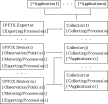
\includegraphics[width=0.7\textwidth]{figures/ipfix-reference-model}
  \end{center}
  \caption{IPFIX Reference Model~\cite{rfc5470}}
  \label{fig:ipfix_reference_model}
\end{figure}

Although the IPFIX Reference Model describes the flow monitoring architecture in detail, it is not used by the flow monitoring community unanimously. Most of the terms used in the IPFIX standard are simplified and their true meaning often depends on the context. Table~\ref{tab:flow_monitoring_terminology} provides the common terms often used instead of the IPFIX terminology. Examples of use of the \Index{common terminology} can be found for example in~\cite{Hofstede-2014-Flow, Cejka-2015-Using, Brownlee-2011-Flow, Krmicek-2009-Netflow, Lee-2007-End, Lee-2007-IPv6, Molina-2006-Design}. We usually talk about a monitored link and a set of monitored links (e.g. both directions of a network connection when optical fibres are used) instead of an observation point or an observation domain. By an exporter or a flow exporter is usually meant the software that performs flow monitoring (both metering and exporting process). If a device generates flows without observing and processing the packets first (i.e. Exporter in IPFIX terminology) we call it a flow source or a probe. The IPFIX Device is usually called by more specific name, such as switch, router, or, in case of a dedicated device possibly with specialized hardware and software equipment, a probe. However, term flow source can also be used for any device that generates flow records. Finally, both the software for collecting flow records and device where such a software runs is commonly called a collector, or a flow collector. We will be using the common terminology throughout this thesis.

\begin{table}[t!]
	\centering
	\begin{tabular}{ll}
	\toprule
		\textbf{IPFIX Terminology}  & \textbf{Common Terminology}                 \\ \midrule
		Observation Point   &  Monitored Link, Observed Link                      \\
		Observation Domain  &  Set of Monitored Links                             \\
		Packet Treatment    &  Packet Treatment                                   \\
		Metering Process    &  (Flow) Exporter [software]                         \\
		Exporting Process   &  (Flow) Exporter [software]                         \\
		Exporter            &  Flow Source, (Flow) Probe                          \\
		IPFIX Device        &  Flow Source, (Flow) Probe, Switch, Router, \ldots  \\
		Collecting Process  &  (Flow) Collector [software]                        \\
		Collector           &  (Flow) Collector [device]                          \\ \bottomrule
	\end{tabular}
	\caption{Flow Monitoring Architecture Terminology}
	\label{tab:flow_monitoring_terminology}
\end{table}


\subsection{Flow Monitoring Deployment}

The deployment of flow monitoring requires careful planning so that it does not disturb the existing network infrastructure. There are several decision that must be made such as choosing a proper flow source, collector and their location relative to the monitored network. Although it is possible to monitor wireless and virtual networks, we focus on the deployment in wired networks.

The selection of the flow source depends upon many variables, such as cost, required quality of exported data, or the type of the monitored link. Two types of flow source are generally available. First are the active networking devices that are already present in the network and provide flow monitoring functionality as well. Switches, routers and firewalls belong to this category. When such a device is present at a convenient point in the network, it must only be properly configured for flow export and no adjustments to the network are needed. Moreover, internal information such as IP addresses behind NAT (Network Address Translation), which would be difficult to access otherwise, can be added to exported flow records. The disadvantage of these devices is that flow monitoring is not their primary function and may not be performed correctly under great load (i.e. under an attack). Also the range of supported options and protocols is usually much lower than that of dedicated probes. The reason for deploying a dedicated probe is usually the need for some extra functionality or guarantees that cannot be met by the networking devices. It also allows to separate network configuration and maintenance from network monitoring, which can be useful if they are handled by different divisions of an organization.

The active networking devices observe packets as a part of their function, dedicated probes, however, need to be provided with access to data. There are two ways for probes to observe the data: in \emph{in-line} mode or \emph{mirrored} mode.
\begin{description}
	\item[In-line mode] -- A device in in-line mode is connected directly to the monitored link and has to actively pass the packets in order for the link to function. This is the mode of operation of active network devices such as switches and routers. The advantage is that no other device is necessary to mirror the traffic, however, if the probe fails the operation of the network is disrupted. Moreover, it could introduce significant latency and jitter to the network connection.
	\item[Mirrored mode] -- In the mirrored mode, a copy of network traffic is created and delivered to the probe using dedicated link. The copy can be created either by dedicated TAP (Test Access Point) or an active networking device with the use of a SPAN (Switch Port Analyzer) port. Table~\ref{tab:tap_vs_span} shows differences, advantages, and disadvantages of TAP and SPAN solutions. An analysis of traffic trace artefacts caused by port mirroring was performed by~\citeauthor{Zhang-2007-Traffic} in~\cite{Zhang-2007-Traffic}.
	\begin{description}
		\item[TAP] is a passive splitting mechanism which require in-line installation. However, due to the simplicity of the device (optical TAPs use mirrors and require no power source) and integrated fail-safes (bypass TAPs), the risk of negatively affecting the network is very low. 
		\item[SPAN] is a special port provided by active networking device that provides a copy of traffic passing through the device for analysis and monitoring purposes.
	\end{description}
\end{description}

\begin{table}[t!]
	\centering
	\begin{tabularx}{\textwidth}{XX}
	\toprule
		\multicolumn{1}{c}{\textbf{TAP}}  & \multicolumn{1}{c}{\textbf{SPAN}} \\ \midrule[1pt]
		
		\multicolumn{2}{c}{Differences} \\ \midrule
		\begin{compactitem}
			\item RX \& TX signal delivered on separate ports
			\item Captures everything on the wire, including MAC and media errors
			\item Complete capture for 100\,\% saturated network
		\end{compactitem}
		&
		\begin{compactitem}
			\item RX \& TX copied into in one TX signal
			\item Hardware and media errors are dropped
			\item Possible packet drop due to SPAN link capacity limit
		\end{compactitem}
		\\ \midrule
		
		\multicolumn{2}{c}{Advantages} \\ \midrule
		\begin{compactitem}
			\item Monitoring device receives identical data, including errors
			\item Keeps link directions separate
		\end{compactitem}
		& 
		\begin{compactitem}
			\item Low cost 
			\item No changes to network topology
			\item Aggregation of multiple links
		\end{compactitem}
		\\ \midrule
		
		\multicolumn{2}{c}{Disadvantages} \\ \midrule
		\begin{compactitem}
			\item Analysis device may need dual-port capture interface
			\item Additional costs for TAP
			\item Necessity to install additional device
		\end{compactitem}
		& 
		\begin{compactitem}
			\item Packet drop on fully utilized full-duplex links
			\item SPAN port data has lower priority than port-to-port data
			\item Some analyses require observation of physical layer errors
			\item Loss of information about link
			\item Increased switch CPU utilization
			\item Can change a timing of frames
		\end{compactitem}
		\\ \bottomrule
	\end{tabularx}
	\caption{Differences Between TAP and SPAN Mirroring Options}
	\label{tab:tap_vs_span}
\end{table}

Since flow monitoring is a passive form of monitoring in its nature, it is a good practice to mirror the live traffic and provide only a copy of the data to the probe so that the network cannot be affected by the monitoring process. Selection of the mirroring technology needs to be considered for each deployment based on specific requirements and limitations, such as utilization of the measured network and impact of packet drop on the performed analysis. The Figure~\ref{fig:flow_monitoring_deployment} shows the most common deployment of flow monitoring at the edge of the network using both presented options: flow export directly from the router and dedicated probe with data provided either by TAP or by router SPAN port.

\begin{figure}[t!]
  \begin{center}
    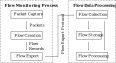
\includegraphics[]{figures/flow-monitoring-deployment}
  \end{center}
  \caption{Flow Monitoring Deployment Schema}
  \label{fig:flow_monitoring_deployment}
\end{figure}

Location of the flow source in the network is very important. When the monitored network is connected to the outside at multiple points, it is necessary not only to monitor each of the points, but also to be sure that the routing policies are reasonable so that packets of each flow traverse only one of these points. The flow source would have to have access to all links and monitor them as a single source otherwise, which is not easily achieved especially when the connection points are geologically distributed. It is a good practice to keep the information about which flow source exported which flow records on the collector so that possible configuration problems are easier to detect.

When monitoring a large network such as a network of an university campus, multiple flow sources can be utilized to gain more detailed information about traffic of individual faculties. Special care needs to be taken when a packet traverses multiple observation points. Counting the same traffic multiple times can have a negative impact on subsequent data analysis.

Deployment of NAT impedes network visibility. Some routers that perform the address translation are able to export both original and translated addresses in the flow records. However, observation points of dedicated flow probes are located either before or after the network device which performs the translation. Although some effort has been dedicated to detection of NAT from data provided in flow records~\cite{Abt-2013-Passive, Krmicek-2009-Netflow}, if does not solve the problem of finding the correct source of the communication behind the NAT. The correct approach would be to either place a second probe to a location where the internal addresses are still visible or to export the information about translation to the collector and pair it with existing flow records.


\section{Flow Monitoring Process}\label{sec:flow-monitoring-process}

This section aims to describe the process of converting raw packets and corresponding packet treatment information to flow records. We show how the flow selection function from Definition~\ref{def:flow-selection-function} relates to this process. For the purposes of this thesis, we will consider dedicated probes equipped with a flow exporter software from now on. Although the the flow monitoring process in networking devices is similar, it has differences and specifics that are outside the scope of this work. This section provides generic overview of the flow monitoring process, performance related details are left for Chapter~\ref{chap:flow-monitoring-performance}.

The Figure~\ref{fig:flow_monitoring_process_detail} shows a common flow monitoring process and its individual parts, which are discussed in the rest of this section. Alternative description of the flow monitoring process can be found in the IPFIX Reference Model~\cite{rfc5470}. We will refer to this description where appropriate.

\begin{sidewaysfigure}
  \begin{center}
    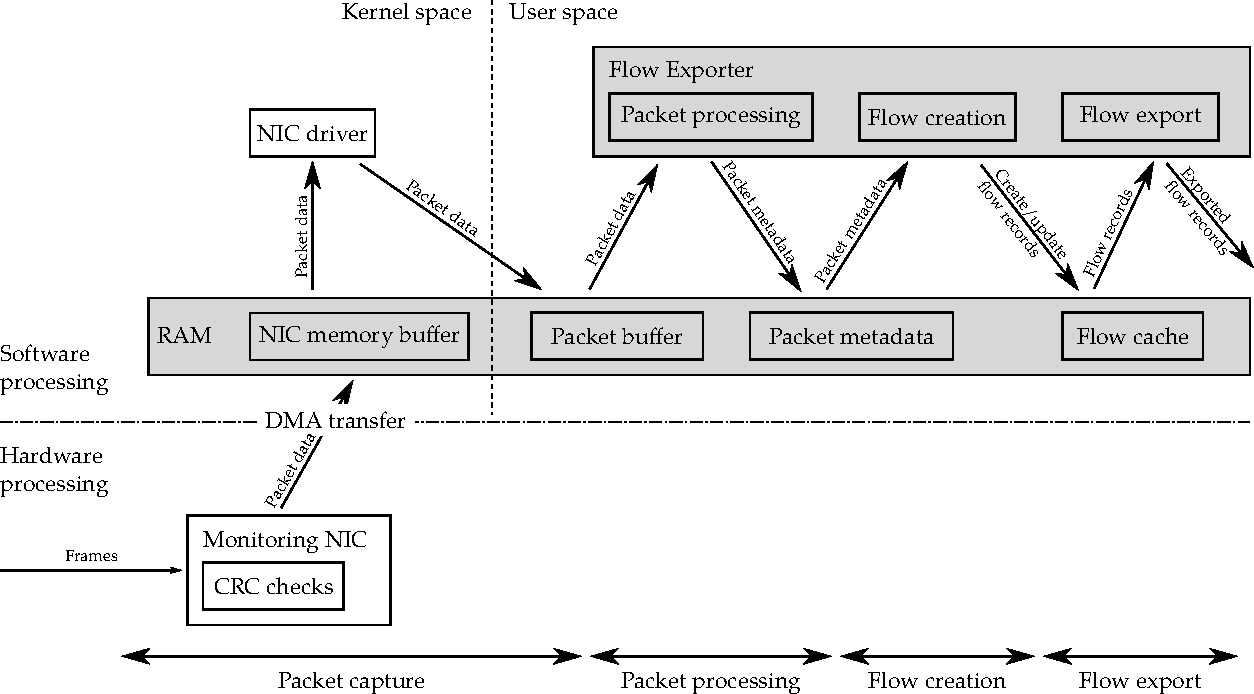
\includegraphics[width=\textheight]{figures/flow-monitoring-process-detail}
  \end{center}
  \caption{Detailed Overview of the Flow Monitoring Process in a Dedicated Probe}
  \label{fig:flow_monitoring_process_detail}
\end{sidewaysfigure}

\subsection{Packet Capture}

The \Index{packet capture} ensures that data from the network are made available for processing in the software. Standard Network Interface Cards (NICs) can be used, as well as specialized hardware accelerated cards. The schema shows a standard NIC performing a CRC check on received packets. The NIC has to be put in a special monitoring mode in order to receive packets with different destination MAC addresses. These packets are passed to the NIC driver, usually through Direct Memory Access (DMA). The driver either passes the received packets to the operating system or provides it's own application interface for accessing the packets from user space. The performance of the different approaches differ significantly and we will discuss it in Chapter~\ref{chap:flow-monitoring-performance} in detail.

Each packet needs to be assigned a (preferably unique) timestamp that marks the point in time at which the packet was received. This process is called packet timestamping. The timestamp can be assigned by the NIC, NIC's driver (or OS), or the software application processing the packet. The support for NIC timestamping is provided by some of the hardware accelerated NICs. As the timestamping in software can be potentially computationally intensive, we will also discuss it in Chapter~\ref{chap:flow-monitoring-performance}.

The packet treatment information is provided together with the packets by the NIC's driver. Usually the interface of NIC on which the packet was captured and the timestamp of the capture is available at least. Networking devices can provide more information such as egress interface, next hop, or autonomous system number of the destination. This information is not directly available when dedicated probes are used, but can be added externally if necessary.

\subsection{Packet Processing}\label{subsec:packet-processing}

The task of the \Index{packet processing} is to extract values of chosen properties of individual packets and corresponding packet treatment information. Attributes such as IP addresses, transport protocol, and ports are used as \emph{flow keys}. The set of used flow keys depend on the applied flow selection function which is used to decide to which flow the packet belongs to. Other attributes of the packets such as TCP flags or number of bytes, are extracted as well for further analysis. We call the extracted properties \emph{\Index{packet metadata}} or \emph{\Index{partial flow records}}. The packet metadata are passed to flow creation part of the flow processing where it is used to create new or update existing flow records.

Secondary task of packet processing is packet sampling and packet filtering, as mentioned in~\cite{rfc5470}. Packet sampling is usually done to reduce the amount of processed data in order to compensate for lack of performance. There are several sampling techniques that can be used as described in~\cite{rfc5476}. Packet sampling is performed before extracting the metadata. Packet filtering can be performed after the metadata is extracted and is based on the extracted values. It is common to monitor only specific network or a section of network, therefore the filtering rules are usually based on extracted IP addresses. Both packet sampling and packet filtering can be implemented in hardware accelerated NICs as well.

\subsection{Flow Creation}\label{subsec:flow-creation}

The extracted packet metadata are aggregated to create flow records. The definition of the flow selection function requires all preceding extended packets of the same flow to determine whether a new packet belongs to particular flow. Since it is not viable to keep all packets of a flow in memory, only selected information is stored in real world implementations. All active flows have a flow record with all the necessary information stored in a \emph{\Index{flow cache}}. When a new packet arrives, the flow selection function is called for each stored flow record and the metadata of the new packet to determine, to which flow the new packet belongs. If a matching flow record is found, it is updated using the packet metadata (e.g. packet and byte counters are incremented, and the flow end timestamp is updated). If no such record exists, the packet is considered to be the first packet of a new flow and a corresponding flow record is created in the flow cache. Algorithm~\ref{alg:flow-record-construction} illustrates the flow creation process. It is worth noting that the flow selection function is denoted $\phi$ as we refer to a concrete implementation here instead of the formal definition.

\begin{algorithm}
    \caption{Construction of flow records}
    \label{alg:flow-record-construction}
    \begin{algorithmic}[1]
        \LOOP 
            \STATE Get new packet $P$
            \STATE Extract packet metadata $M$
            \STATE Set \textbf{found} = \FALSE
            \FORALL{flow record $\mathcal{F}$ in flow cache}
                \STATE Apply flow selection function $\phi$ to $\mathcal{F}$ and $M$
                \IF{$\phi(\mathcal{F}, {M}) = true$}
                    \STATE Aggregate $M$ to $\mathcal{F}$
                    \STATE Set \textbf{found} = \TRUE;
                    \STATE \textbf{break}
                \ENDIF
            \ENDFOR
            \IF{\NOT found}
                \STATE Create new flow record $\mathcal{F}$ from $M$
                \STATE Insert $\mathcal{F}$ into flow cache
            \ENDIF
        \ENDLOOP
    \end{algorithmic}
\end{algorithm}

Testing the extracted packet metadata against each flow record has a linear time complexity with respect to to the size of the flow cache. Common optimization is to compute a hash for each flow record such that it can also be computed for the extracted metadata. The flow cache is then either indexed by using the computed hash~\cite{Molina-2006-Design} or directly implemented as a hash table~\cite{Estan-2004-Building} so that the input and lookup operations have a constant time complexity. Collisions can be solved by a number of common techniques or by prematurely exporting the older colliding flow record. This optimization is so widely used that its use is often implicit, but it is important to keep in mind that the new packet is still effectively tested against each active flow. Other implementations of flow caches can be found in literature, such as a hypercube flow table by~\citeauthor{Wang-2011-Memory}~\cite{Wang-2011-Memory}.

There are several reasons why a flow record can exit the flow cache\index{flow!record expiration}{}:
\begin{description}
    \item[Inactive timeout\index{timeout!inactive}] occurs when no new packets belonging to the flow arrive for a time interval called \emph{inactive timeout}. This timeout is used to end inactive connections and has a significant influence on flow cache memory requirements. When set too low the inactive timeout can erroneously split idle connections where keep-alive packet are sent in a longer interval than the inactive timeout. The inactive timeout is sometimes called \emph{idle timeout}\index{timeout!idle} as well.
    \item[Active timeout\index{timeout!active}] occurs when the flow is longer than a time interval called \emph{active timeout}. The reason for active timeout is to keep exported flow information fresh. For example some SSH connections may be active for months when left open in an UNIX/Linux screen utility and without the active timeout the information about the connection would be too late for any practical purpose, such as monitoring the amount of traffic for a given time period. The active timeout is usually much longer than the inactive one. For example, Cisco IOS flow cache has the default of 30 minutes for the active timeout and 15 seconds for the inactive one~\cite{CiscoSystems-2013-Cisco}.
    \item[Natural expiration] occurs when the connection is closed normally. This is often implemented for TCP connections where packets with RST or FIN flag indicate the end of connection.
    \item[Resource constraints] such as lack of memory can cause flow records to be exported from the flow cache to allow new flows to be inserted. Some implementations of flow caches using hash tables have fixed number of flows that can be stored under single hash. Therefore, when a new flow record needs to be created one of the existing flow records is usually expired.
    \item[Exporter shutdown] usually causes all flow records in the flow cache to be exported so that the information about observed packets is not lost. This cause is not often mentioned in the literature, however, we consider it an important one. The exporter must be restarted each time a configuration is changed unless it supports dynamic reconfiguration, which none of the open-source exporters does. Therefore the exported shutdown can happen surprisingly often.
\end{description}

The RFC 5470~\cite{rfc5470} considers both timeouts and resource constraints as causes for a flow record to expire but omits natural close of connection and the possibility of exporter shutdown. Flow record expiration setting can significantly influence not only the  number of generated flow records, as shown by the authors of~\cite{Rodriguez-2013-Empirical}, but also further flow processing and various flow-based detection methods. Implementation of flow record expiration has an impact on the overall flow monitoring performance. Periodically checking the flow cache for expired flows can create latency in packet capture that may result in packet loss. Several approaches to this problem are described in the work of \citeauthor{Molina-2006-Design}~\cite{Molina-2006-Design}.

% On the impact of TCP segmentation: Experience in VoIP monitoring by D. Muelas et al.; and Low-cost and high-performance: VoIP monitoring and full-data retention at multi-Gb/s rates using commodity hardware, by J.L. García-Dorado et al. 
% Both works cope with this matter, and provide some insights that may extend the discussion in the manuscript.

Little attention has been given to the measurement of traffic with fragmented packets. Although the ratio of fragmented packets is decreasing~\cite{Murray-2012-State}, it is still very important to monitor them since it is quite easy for an attacker to hide an attack from intrusion detection systems by fragmenting the attack packets~\cite{Cheng-2012-Evasion}. The RFC 3917 which describes requirement for IP flow information export states the following about packet fragmentation:

\begin{displaycquote}{rfc3917}[Requirements for IP Flow Information Export (IPFIX)]
   In case of IP packet fragmentation and depending on the
   classification scheme, only the zero-offset fragment of a single
   initial packet might contain sufficient information to classify the
   packet.  Note that this fragment should be the first one generated by
   the router imposing the fragmentation [RFC791], but might not be the
   first one observed by the IPFIX device, due to reordering reasons.
   The metering process may keep state of IP packet fragmentation in
   order to map fragments that do not contain sufficient header
   information correctly to flows.
\end{displaycquote}

This means that the flow monitoring system implementing the IPFIX standard is not required to handle fragmented packets. Moreover, neither the Netflow v9 nor the IPFIX flow definitions cover the possibility to assign a packet fragment to the correct flow, because they require that the common properties are derived from the single packet and the corresponding packet treatment. This is the main reason that the Definitions~\ref{def:flow} and~\ref{def:formal-flow} allow to derive the common properties from data contained in previous packets of the same flow as well. We assume that the packets arrive in the appropriate order for the purpose of these definitions.

Let us consider what happens when an IPv4 packet is fragmented (the problem is very similar for IPv6). Figure~\ref{fig:fragmented-flow} illustrates this scenario. When the packet $K$ is fragmented, its payload is distributed between several different packets $(K\#1, K\#2, \ldots, K\#M_K)$. Only the first packet $(K\#1)$ contains the transport header, others only carry a flag identifying the fragment and offset of the data in the original packet. When a flow record is created for the first part of the fragmented packet, it contains IP addresses, transport layer information (protocol and ports), and the first part of application payload. However, subsequent parts contain only information about IP addresses and consecutive parts of the application payload. The transport level information was already sent in the first fragment. Therefore, flow records created from the subsequent fragments are not aggregated with the first fragment. Moreover, flow records created from subsequent fragments from different connections between the same hosts are aggregated together. To resolve this problem, some kind of packet reassembly must happen either in the flow cache or during packet capture (e.g. packet reassembly at the OS network stack).

A possible solution that has been successfully deployed in practice is to create temporary flow records for fragmented packets where fragmentation identifiers are part of the flow key instead of transport layer information. Therefore, each fragmented packet has its own temporary flow record. By assigning shorter inactive timeout to these flow records the temporary flow record can be reinserted into the flow cache when all fragments are received. This allows to effectively reassemble the original packet with proper transport layer information, which is available since it was present in the first fragment, in the flow cache. The advantage of this solution is that it allows to count number of reassembled packets as well as the number of packet fragments, which can be used in later analyses.

\begin{figure}[ht!]
  \begin{center}
    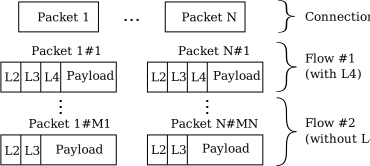
\includegraphics{figures/fragmented-flow}
  \end{center}
  \caption{Flow measurement of a fragmented connection.}
  \label{fig:fragmented-flow}
\end{figure}

The flow monitoring implementation based on flow caches of networking devices kept a separate flow for each direction of a network connection. The reason was that each direction usually had different at least  ingress and egress interfaces. However, for network monitoring and analysis purposes, it is often useful to be able to access flow records for both communication directions at the same time. For this reason the bidirectional flow export was proposed in 2005 and resulted in publication of RFC 5103~\cite{rfc5103} in 2008. The document proposes to aggregate flow records for both forward and reverse directions to a single flow record. Bidirectional flow is called \emph{\Index{biflow}} and unidirectional flow is called \emph{\Index{uniflow}}. The flow keys that are associated with a direction (e.g. source IP address) are called \emph{directional flow keys}. When the biflow record is created, some information must be stored for both directions (e.g. number of bytes and packets) and some information is common to both directions (e.g. flow keys). When biflows are used, the corresponding flow records stored in the flow cache become biflow records as well. Note that creation of biflows is permitted by the definitions NetFlow v9 and IPFIX as well as the Definition~\ref{def:flow}. Although we work mostly with the uniflow in the context of this thesis, most of the concepts apply to the biflow as well. We will mention explicitly when there are important differences between uniflow and biflow.

\subsection{Flow Export}

The flow export manages the process of delivering flow records to flow collectors. The process consists of several parts as shown in the Figure~\ref{fig:flow-export}. The flow sampling and filtering process is very similar to packet sampling and filtering described in the Subsection~\ref{subsec:packet-processing}. The main motivation for flow filtering is that each collector might want to process only a subset of data, e.g. from a particular subnet. The flow sampling is performed when the performance of the collector is not sufficient to process all flow records. The main difference between packet sampling and flow sampling is that the flow sampling always discards whole flow record while the packet sampling can discard some packets of the flow, therefore affecting the created flow record. 

\begin{figure}[ht!]
  \begin{center}
    \includegraphics[width=\textwidth]{figures/flow-export}
  \end{center}
  \caption{Flow export schema.}
  \label{fig:flow-export}
\end{figure}

The flow export protocols such as NetFlow or IPFIX describe how to serialize a flow record and how to use different transport protocols such as UDP, TCP and SCTP to transfer the encoded data to the collector. The NetFlow~v5 and v9 protocols are still widely used although the IPFIX protocol is achieving wide deployment since it offers more features and supports proprietary information elements as well as variable length information elements. Different flow export protocols developed by other vendors can be used as well, as described in Subsection~\ref{subsec:history-of-flow-monitoring}.

The UDP transport protocol is used very often to carry flow records since it was the only one supported by NetFlow. IPFIX specifies the use of TCP and SCTP protocols for flow export as well as the use of the UDP protocol. Although SCTP is mandatory for IPFIX implementations, its real-world usage is hindered by lack of support in software and hardware. When a reliable transport is necessary, TCP is the most often used protocol. For more information about IPFIX transport protocols see RFC 7011~\cite{rfc7011}. A comprehensive comparison of IPFIX transport protocols is also provided in~\cite{Hofstede-2014-Flow}.

Flow records can be exported in many formats over different transport protocols. With the increasing popularity of big data tools such as Kafka, Elasticsearch, Apache Spark, and Hadoop, the need for an universal and widely supported format is more crucial then ever before. As most of the big data tools support JSON, flow records are often transported and stored in the JSON format. The main advantage of JSON is that the data are stored in key-value format without the need to specify templates for the data beforehand. The obvious disadvantage is the increase in the message size due to the need to provide a key for every value in every flow record. It is not unusual for the JSON encoded messages to be more than 7 times larger than in the IPFIX format.

An important part of flow export is ensuring security of the exported flow records. The records must reach only the authorized destination without being observed by any third party. Therefore, authorization, confidentiality and, preferably, also integrity should be provided. The same applies to flow collectors during the collecting process. More information about flow transmission security is provided in Subsection~\ref{subsec:flow-collection}.

\section{Flow Data Processing}\label{sec:flow-data-processing}

The aim of this section is to outline the processing of flow data after they are exported to a flow collector. Firstly, we describe the flow collection process in Subsection~\ref{subsec:flow-collection}. The reception of flow data is not a difficult task itself, but requires several important choices to be made, such as what flow export protocols will be supported and how to handle unknown information elements. Secondly, the flow data are often stored for future needs. The choice of a flow data storage format is very important since the data is written once, read many times and fast searches are required. This process is described in Subsection~\ref{subsec:flow-storage}. Lastly, the flow records are processed and analysed, either by reading the previously stored data or in real time as they arrive from a flow exporter. The flow record processing and analysis is discussed in Subsection~\ref{subsec:flow-processing}. The whole flow data processing schema is shown in Figure~\ref{fig:flow-processing-details}.

\begin{sidewaysfigure}
  \begin{center}
    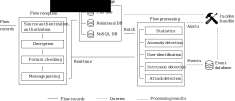
\includegraphics[width=\textheight]{figures/flow-processing-details}
  \end{center}
  \caption{Flow data processing schema.}
  \label{fig:flow-processing-details}
\end{sidewaysfigure}

\subsection{Flow Collection}\label{subsec:flow-collection}

Flow collection is a process of receiving flow records from an exporter performed by a flow collector. The collector and the exporter must choose an appropriate combination of transport protocol and flow export protocol before the data transmission starts, there is no protocol for flow export parameters negotiation. Although the collector can receive data using a multiple combinations of protocols at the same time, such feature is not usually implemented due to added complexity.

After the collector validates that a received message is in the expected format, it attempts to parse individual flow records. This process may vary for each flow export protocol, however, the collector always needs to derive correct data types of information elements in order to be able to work with them. The common practice with NetFlow information elements was to hardcode their definitions and extend the code every time it was necessary to add a new element. The extensibility of the IPFIX protocol information elements through the use of Private Enterprise Numbers advocates more dynamic approach to information element handling, although a subset of IPFIX information elements are sometimes hardcoded as well. Since the collectors cannot know all possible information elements that can be sent by exporters, it is necessary to correctly handle new and unknown elements. Although they are usually discarded, it is also possible to process them when their data types can be derived from the information provided by the flow export protocol.

When using NetFlow and IPFIX protocols in combination with the UDP transport protocol it is necessary to properly manage templates messages containing the definitions of flow record formats. The templates can change during the collection process, e.g. after exporter restart, and it can easily result in incorrectly decoded messages. The IPFIX protocol specification~\cite{rfc7011} describes how the template messages should be handled and what to do in case of missing templates. Both NetFlow and IPFIX protocols keep track of lost messages by assigning a sequence number to each message. NetFlow~v5 increase the sequence number for each transmitted flow record, which allows to keep track of the number of lost flow records. This behaviour was changed in NetFlow~v9 so that the sequence number is increased for each transmitted NetFlow~v9 packet. It is more difficult to keep track of the number of lost flow records in NetFlow v9, but easy to see how many packets were lost, which can help with determining the cause of the packet loss. The IPFIX protocol increments the sequence number per flow record, just like NetFlow~v5. However, when a template is missing, it is not possible to determine the exact number of flow records in a packet, therefore the collector cannot be sure whether flow records were lost during the transmission or not. This is one of several reasons to use IPFIX over a reliable channel.

An important and often neglected aspect of flow collection is security. The collector needs to authenticate the source of the data to avoid processing of malicious flow records or malformed messages intended to attack the collector itself. There are several ways to authenticate the source of the data. IP addresses can be used to authenticate the flow exporter and the collector itself or a firewall can be set to allow data from authorized IP addresses. However, this does not prevent attackers with the ability to spoof IP addresses when UDP transport protocol is used. Moreover, the Man-in-the-middle (MITM) attack cannot be prevented without an appropriate use of cryptography. Proper authentication, usually using certificates, is needed to mitigate the MITM attack. The IPFIX protocol requires that TLS version 1.1 is implemented for TCP and DTLS 1.0 for STCP and UDP procols. Moreover, it requires mutual authentication when using TLS or DTLS so that the exporter does not send sensitive data to an unknown target. Table~\ref{tab:flow.protocols.security} shows how IP spoofing and MITM attack are mitigated by use of TLS and DTLS protocols. The advantage of TLS and DTLS protocols is that they provide not only authentication, but also integrity and confidentiality. Since an IP address is often considered to be a sensitive information, ensuring confidentiality of flow records during transmission should be considered a necessity.

\begin{table}[t!]
	\centering
	\begin{tabular}{lll}
	\toprule
			& \textbf{IP Spoofing}	& \textbf{Man-in-the-Middle}  \\ \midrule
	UDP		& yes			& yes \\ 
	TCP		& no			& yes \\ 
	SCTP		& no			& yes \\
	DTLS/UDP	& no			& no  \\
	TLS/TCP		& no			& no  \\ 
	DTLS/SCTP	& no			& no  \\ \bottomrule
	\end{tabular}
	\caption{Applicability of IP spoofing and MITM attack to transport protocols}
	\label{tab:flow.protocols.security}
\end{table}

Although the IPFIX protocol requires implementation of TLS and DTLS protocols, not every flow exporter and collector supports it. There are two often used solutions for ensuring security of flow record transmission. The first is to build secure channel between exporters and collectors using external tools, such as virtual private networks or stunnel~\cite{Trojnar-2015-Stunnel}. The second solution used in networks that are fully under control of the administrator is to place the exporter and collector in a dedicated network (using private IP addresses) so that they can be accessed only from allowed and trusted address range.


\subsection{Flow Storage}\label{subsec:flow-storage}

There are many uses for flow data~\cite{Li-2013-Review, Umer-2017-Flow}. At first the data were being used for traffic accounting and flow records are often kept by telecommunications companies to comply with laws requiring them to store communication records nowadays. Companies and even individuals also keep flow records of their own traffic so that they can investigate breaches and other security issues ex-post. To store the flow data records for a long period of time, the selected data storage format must be space efficient. Another important aspect of flow data storage is its query performance. The requirements for the query performance differ depending on a particular use case. When overall statistics are requires, all flow records need to be accessed. In case of a security breach investigation, filters for particular IP addresses and ports are likely to be used so that it is beneficial for the data storage to have some kind of index built on the data.

There are several types of data storage that are used for flow data. Firstly, the data can be stored in a flat file without indexes. This approach is utilized by popular flow data manipulation frameworks SiLK~\cite{Shimeall-2014-Using} and NFDUMP~\cite{Haag-2014-NFDUMP}. The main advantage is that the format is very simple and the data is efficiently encoded. Moreover, both file formats support compression which allows for more disk space to be saved. Flat files also take advantage of the fact that flow data is never updated so the records can be tightly packed.

A second popular approach is to store flow data in a relational database. In case of NetFlow~v5, a single table serves to store all flow records. However, when multiple templates are used for the flow records, such as in NetFlow~v9 and IPFIX protocols, the number of tables grows and the relational model becomes complicated. Since relational databases are designed to support much more features than needed for flow data (e.g. updates or complex joins) and often lack support for network data types such as IP and MAC addresses, their performance and disk space requirements are often worse than that of flat files, as shown by \citeauthor{Hofstede-2010-Network} in~\cite{Hofstede-2010-Network}.

The last approach is to use a NoSQL database to store flow data. Although NoSQL databases do not offer as many features as relational databases, they are meant to be able to handle huge amounts of data. A category of NoSQL databases are columnar databases. Instead of storing each flow record as a single database record, it stores each element of the record in a separate file. The benefit of this approach is that, for example, when a query for a certain IP address is evaluated, only files with IP addresses need to be searched. Other requested elements are read from their own files as necessary after the address is found. This approach reduces the amount of data that needs to be read from the disk, however, it causes more random accesses than when using flat files. More information about comparing flat file approach with a NoSQL columnar database is provided in Chapter~\ref{chap:next-generation-flow}. Document oriented databases are also a class of NoSQL databases and their popularity has been increasing lately. Although the performance of most document oriented databases is not sufficient to handle flow data from large networks, they are used for their flexibility that allows for building prototype analytics applications very quickly. The advantage of document oriented databases is that the different structure of flow records is of no concern to the database as it considers each entry to be a generic document. Elasticsearch~\cite{Gormley-2015-Elasticsearch} is a good example of a such a database.

The list of used approaches is by no means complete. There are many Big Data analytics frameworks, that are being used for flow data storage and analytics, such as Hadoop~\cite{Lee-2012-Toward}. Although it is possible to use almost any data storage for flow data, it is difficult to select the best one, since the criteria differ for each use case. It is for that reason, that companies use different flow data storage or develop their own solution in their products.


\subsection{Flow Processing}\label{subsec:flow-processing}

Large amount of information about network traffic and communicating parties can be acquired by a flow record analysis. Many intrusion detection systems use flow records as their primary source of data, especially since deep packet inspection is being made difficult due to the increasing ratio of encrypted traffic. The flow data analysis can be performed either using the stored data or in real time.

When the flow record analysis is performed on stored data, the processing is usually done in batches. The flow collector usually partitions the data according the time of arrival so that once a partition is finished, it can be processed in a single batch. Five minute long time windows are often used as this is the default time interval employed by the popular flow processing tool NfSen~\cite{Haag-2011-NfSen}. The advantage of this approach is that the processing can easily be repeated on the same data, which allows the user to fine-tune the queries and analyse the data on demand. The processing can also be postponed when the system is under heavy load. The disadvantage of batch processing with fixed time intervals is that it introduces delays to data analysis, which can be inconvenient when a rapid action is required based on the results.

When the delay introduced by the batch processing impedes time-critical applications, stream processing can be used instead. In stream processing, the flow records are passed to the processing immediately after they are received. A good overview of the stream-based flow processing is provided by \citeauthor{Jirsik-2017-Toward} in~\cite{Jirsik-2017-Toward}. There is a number of stream processing systems that are used for big data processing. \citeauthor{Cermak-2016-Performance} performed flow data analysis using three most used distributed stream processing systems in~\cite{Cermak-2016-Performance}, and compared their performance. The results show that the distributed stream processing systems are able to scale to accommodate large workloads such as processing of data from very large networks.

The flow processing can be used to achieve several goals. Firstly, both live and long term network statistics can be computed. Live statistics are used by administrators to gain an overview of a network situation. This is useful for tracking down problems and optimizing network configuration when the changes take effect immediately. The long term statistics provide useful information for capacity planning. Secondly, flows can be used to gain situational awareness about the network and connected devices~\cite{Lastovicka-2017-Situational}. This includes device identification and application classification, which often use machine learning techniques for this purpose. Thirdly, flows are nowadays frequently in intrusion detection systems used to detect attackers on network, as described by \citeauthor{Umer-2017-Flow} in~\cite{Umer-2017-Flow}. Lastly, anomaly detection techniques are being applied to flow data to detect suspicious behaviour which might indicate a problem or attack on the network. There are many anomaly detection techniques as surveyed by \citeauthor{Chandola-2009-Anomaly} in~\cite{Chandola-2009-Anomaly} and significant effort was put to applying these techniques to flow data by various researchers.

Modern machine learning techniques are utilized in flow processing. The most common uses are in traffic classification~\cite{Velan-2015-Survey}, user identification~\cite{Verde-2014-No} and intrusion detection~\cite{Tsai-2009-Intrusion}. Although the research in this area is quite extensive, the authors of~\cite{Sommer-2010-Outside} show that the result are seldom applied in practice and provide several observations explaining the difficulties faced by the implementers. A survey of traffic classification techniques for encrypted traffic is provided in Chapter~\ref{chap:measurement-of-encrypted-traffic}.


\section{Common Issues}\label{sec:common-issues}

Although flow monitoring is widely used, there are many not widely known aspects that need to be taken into consideration during its deployment. This section describes several issues that can be encountered in any flow monitoring system and that are easily neglected. We draw mainly from our experience of running the flow monitoring infrastructure of CESNET National Research and Education Network in this section. Most issues concern data loss. Either the data is not correctly observed, parsed, are lost during transmission, or are not interpreted correctly. Firstly, we look at the more obvious and easily detectable issue where no data arrive at all. Then we describe the issues that cause data loss which is not easily detected. Lastly, we discuss issues and misunderstandings that cause the data to be incorrectly measured and interpreted. Let us note here, that a suitable logging facilities of flow exporter and collector together with a reliable log processing mechanism can help to discover many of the described issues.

\subsection{Visible Data Loss}

The usual cause of data loss is that the monitoring infrastructure is misconfigured. Whether it is due to a misconfiguration at the flow exporter or the flow collector side, the obvious indication of the problem is that no data are stored and no results of the flow data processing, such as statistics, are generated. As the problem is quite easily observed, its cause is easily detected. The best way is to review the whole flow processing setup from packet observation to flow storage and processing to see at which point the data are lost.

The first component to investigate is the packet observation. It is possible that the data are no longer sent to the observation point, possibly due to a failed TAP device or a router misconfiguration. This can be easily confirmed using interface packet counters. Even if the data arrive at the observation point, the flow exporter might be configured to read data from from incorrect interface. When the flow exporter is receiving and processing the data, it is important to audit the flow export settings. The data might be sent to incorrect destination or using incompatible transport or flow export protocol. When TLS/DTLS is used, the certificates and keys might not match. It is a good practice to verify that the data actually leave the probe, for example by using a tool such as \emph{tcpdump}.

Since the flow probe is often placed in a dedicated network, it is useful to verify that the network is configured to allow the communication between the probe and the flow collector.

The flow collector must be configured to accept data from the flow exporter, which includes a proper setup of certificates and keys. Even when the flow collector receives the data, it might be running using incorrect configuration and the data might be saved to an unexpected location or not passed to storage and processing at all. A collector may also decide to discard flow records containing unknown information elements. When the flow exporter includes such an element in every record, all flows are dropped. 

\subsection{Unobserved Data Loss}

It is impossible to continuously verify that all observed packets are accounted for in the flow records processed by the flow collector. Since each flow record contains information from packets observed at a different time interval, it is not possible to compute the exact number of packets that passed an observation point from the respective flow data. All statistical information about number of transferred packets are to a certain level biased. The only test that can be continuously applied is that the total number of observed packets at the observation point and at the flow collector remain in a similar range. Since it is not possible to verify that every packet is observed, some packet of even flows might be lost in the flow monitoring process without notice.

There are many networking protocols in use nowadays. Although all flow exporters support the basic protocols such as IPv4, TCP, UDP, and ICMP, they also need to be able to process many data link layer protocols, such as VLAN, VXLAN, MPLS, TRILL, and others. When a new protocol is used on the network for which the flow exporter is not ready, the flow record cannot be created and the information is lost. A similar issue involves tunnelling protocols, such as GRE or protocol 41. For example, when the original IP packet is encapsulated in another L3 protocol, it is important to decide whether the flow record should be created from the inner or outer L3 header. Without an additional mechanism to provide more information about the tunnelled traffic, information from one of the headers is lost.

Flow records containing unknown informational elements might be discarded by the flow collector, as described in the previous section. However, when only some of the flow records contain such information elements, the issue is harder to observe. Therefore it is necessary to have a good knowledge of the used flow collector and its behaviour.

Sometimes messages can be longer than the MTU of the link between the flow exporter and flow collector, especially when application layer information is contained in the flow records. In such a case, use of UDP transport protocol might cause data loss as fragmented packets are sometimes blocked by firewalls. Moreover, the packet loss is more probable since by loosing a single fragment the entire message is unreconstructable and must be discarded. When such a long messages need to be sent, it is best to use a reliable transport protocol such as TCP or SCTP.

One of the most common reasons for data loss in flow monitoring is that the performance of flow exporter or a flow collector is not high enough to process all data. There are several places where either packets or flow records might be dropped, as shown in Figure~\ref{fig:flow-packet-drop}. The first is the source of data for the observation point. When the data to the observation point are provided using router SPAN port, the capacity of the SPAN port must be equal or greater to that of individual links that are measured, otherwise some packet will be dropped by the router when there is a lot of traffic. This is not an issue when using a TAP, because the TAP always splits a single link or a duplex link to two links of the same type and capacity. The second point where packets are often dropped is the observation point. When the exporter does not process the data before the packet reception buffer is full, the newly arrived or the oldest packets are dropped, based on the implementation of the buffer. The third point where the data might be dropped is on the collector device. When the flow collector does not process data quickly enough, the system packet reception buffers fill up and new packets are dropped. This is similar to the packet drop on flow probe, however, every packet lost at the collector contains several flow records that were created from many packets. Therefore, loss of packets with complete flow records is much more serious.

\begin{figure}[t!]
  \begin{center}
    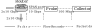
\includegraphics{figures/flow-packet-drop}
  \end{center}
  \caption{Flow monitoring packet drop schema.}
  \label{fig:flow-packet-drop}
\end{figure}

The choice of transport protocol have an impact on the packet drop as well. UDP messages are discarded by the collector when it does not process in a timely manner. However, using congestion aware protocol such as TCP and SCTP, the collector might create a backpressure on the flow exporter so that it cannot send new messages when it needs to. Therefore,the flow exporter can either drop such messages or wait for the collector to process more data. However, when the flow exporter does not drop the messages, it creates backpressure to flow cache, packet processing, packet parsing and packet reception. This way the slow processing on collector might easily lead to packet drop at the observation point. Another reason for flow exporter not being able to send messages is a slow link between the exporter and collector. When application information is present in the flow records, the required throughput might easily exceed 100\,Mbps, especially when the exporter sends data to multiple collectors. Although such slow links are not used very often nowadays, they might still be encountered in practice.

Although packet drop should be avoided at both flow exporter and flow collector sides, sometimes it is necessary to drop packets in a controlled manner, e.g. under a DDoS attack. We recommend to create a packet buffer in the application to which the data is always stored. Then, when the data processing is slow and the buffer becomes full, the application can decide which packets to drop. The advantage of this approach is that the application is aware of the congestion and can properly react to it, e.g. by reporting it or limiting the processing to a bare minimum.

A very common cause of packet loss at the collector side is the shutdown or restart of flow exporter. The flow exporter usually expires all flow records in the flow cache so that they are not lost. However, as the flow cache may contain hundreds of thousands of flow records, exporting them all at one at the highest possible rate (the flow exporter needs to shutdown or restart without an unnecessary delay) can overwhelm the flow collector. Therefore, it is best to implement two types of shutdown, emergency and graceful. In the emergency shutdown, the data in the flow cache are simply discarded as they are not considered important. This allows to quickly shutdown and restart the exporter, which is beneficial during testing and for important configuration changes. The graceful shutdown should have a configurable flow record export rate. This allows to adapt the capabilities of the flow collector without overwhelming it and limiting the risk of data loss.

Flow monitoring performance is discussed in detail in Chapter~\ref{chap:flow-monitoring-performance}.


\subsection{Other Issues}

There are other problems that can be encountered during flow monitoring apart from the performance issues and data loss. We have already described the problem with counting lost flow records and elements in The Subsection~\ref{subsec:flow-collection}. This section describes the most common of the issues that cause the data to be incomplete or incorrect.

The first issue is encountered at flow exporters that process biflows. To process biflows correctly, the exporter needs to observe both directions of each flow. There are several reasons why it may fail to do so. Only single direction might be connected to the probe or the network configuration might route the packets asymmetrically. Even if both directions can be observed at the observation point, packets might be received, parsed, and processed in several different queues to speed up the monitoring process. In such a case, it is important to use a correct algorithm to select queues for packets, otherwise the packets from opposite directions may end up in different flow caches and the created biflows will be incomplete. The algorithm must be able to work with all packet headers that precede the headers from which the flow keys are derived. 

Both the flow exporter and flow collector must agree on the semantics of the elements of exported flow records. For example, the packet length is usually exported in IPFIX format as a \emph{octetDeltaCount} element. The specification~\cite{IANA-2017-IP} defines it to be the number of octets since the previous report (if any) in incoming packets for this Flow at the Observation Point. The number of octets includes IP header(s) and IP payload. However, some exporters put the total number of octets including the link layer in this field. Moreover, the IPFIX protocol is sometimes used to export information about non-IP flows as well, so that this element is used differently for specification. Whether the exporter and collector adhere to the specification, it is important the they interpret the semantics equally. In this case, it would be proper to setup a different element with different semantics if the total number of octets needs to be reported.

Different exporters can encode flow record elements to integers, strings and byte arrays of different length. For example, the IPFIX protocol supports \emph{Reduced-Size Encoding}~\cite{rfc7011} which allows encoding elements using fewer octets than the number specified by~\cite{IANA-2017-IP}. Although this saves resources such as memory of the flow exporter, network bandwidth, and disk space on collector, it makes it more difficult to process correctly. When the same element is received by the collector using two different data types, it needs to decide which is going to be used for further processing as maintaining both original data types is cumbersome. The collector usually converts the data to the largest possible data type since it cannot know it advance whether it will receive the element encoded differently in the future and reducing the size of an element may lead to information loss.

The encoding of TCP flags in IPFIX protocol is a good example of issues that can be caused by the \emph{Reduced-size Encoding}. NetFlow~v9 defined TCP flags element as one byte and the IPFIX used single byte as well originally. However, the TCP control bits occupy 9 bites in the TCP header~\cite{rfc3540}, therefore a change was proposed in 2013 to change the encoding to two bytes. The discussion resulted in RFC 7125~\cite{rfc7125} in 2014 with IPFIX supporting the export of TCP flags as a two byte value, as shown in Figure~\ref{fig:tcp-flags}. When reduced size encoding is used only the original byte is exported for backwards compatibility. This presents the authors of flow collectors with a difficult issue. If they support TCP flags as a two byte value, they must indicate that the received element was only a single byte long. Storing two byte value and padding with zeroes is not an option since that would set the ECN nonce sum flag to zero although the collector has no knowledge of its original value.

\begin{figure}
  \begin{center}
    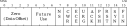
\includegraphics[width=\textwidth]{figures/tcp-flags}
  \end{center}
  \caption{TCP control bits export in IPFIX protocol~\cite{rfc7125}.}
  \label{fig:tcp-flags}
\end{figure}


\section{Summary}\label{sec:nfm-summary}

This chapter has explained flow monitoring, its history, common uses, and discussed related technologies that are sometimes confused with flow monitoring. We have shown, that the currently used definitions of flow do not reflect the reality of real-world flow monitoring deployment and provided and improved definition that amends the deficiencies. We have also created a formal notation for our definition which allows us to avoid misunderstandings created by the use of informal language. It also allows flow related algorithms to be written more precisely and concisely.

The rest of the chapter has discussed details of the flow monitoring process from the packet capture on a probe to the flow processing on a collector. We have also shown the most common issues that can be encountered while deploying and operating a flow monitoring infrastructure. The most critical issues are caused by incorrect implementation and low performance. We investigate the performance of flow monitoring in Chapter~\ref{chap:flow-monitoring-performance}.


\chapter{Application Flow Monitoring}\label{chap:application-flow-monitoring}

\begin{chapintro}

Deep packet inspection (DPI) and basic flow monitoring are frequently used network monitoring approaches nowadays. Although the DPI provides application visibility, detailed examination of every packet is computationally too intensive to be performed on high-speed networks. The basic flow monitoring achieves high performance by processing only packet headers but provides no details about the traffic content. Application flow monitoring is proposed as an attempt to combine DPI accuracy and basic flow monitoring performance. The aim of this chapter is to provide complete information about application flow monitoring. 

The contribution of this chapter is threefold. Firstly, it provides an overview of the current state of application flow monitoring. Secondly, it defines consistent terminology and provides a practical definition of application flow and application flow record. The third contribution is an experimental study of an HTTP parser design. Despite extensive work, flow exporters generally fall short of performance goals due to extracting application layer data. Constructing efficient protocol parser for in-depth analysis is a challenging and error-prone affair. We designed and evaluated several HTTP protocol parsers representing current state-of-the-art approaches used in today's flow exporters. We show the packet rates achieved by respective parsers, including the throughput decrease (performance implications of application parser) which is of the utmost importance for high-speed deployments. The presented results provide researchers and network operators with important insight into application flow monitoring performance.

The paper included in this chapter is~\cite{Velan-2013-Design}, another paper related to this chapter is~\cite{Velan-2014-Next}.

The organisation of this chapter is as follows:
\begin{itemize}
  \item Section~\ref{sec:app-motivation} provides motivation for processing the application layer in the flow monitoring.
  \item Section~\ref{sec:app-rel-work} outlines the state-of-the-art in the field of application flow monitoring.
  \item Section~\ref{sec:app-flow-definition} defines necessary terminology and provides a definition of application flow and application flow record.
  \item Section~\ref{sec:creating-application-flow} describes how the application layer processing affects the flow monitoring.
  \item Section~\ref{sec:http-parser-design} is a case study of an HTTP parser design and of the effect of processing the HTTP protocol on the flow monitoring process.
  \item Section~\ref{sec:app-summary} summarizes the chapter.
\end{itemize}

\end{chapintro}

\newpage

\section{Motivation}\label{sec:app-motivation}

The number of different applications communicating over the Internet is ever increasing, and so is the need for application-aware network monitoring. However, building network monitoring systems is always a compromise between accuracy and performance. The more detailed the information processing, the more accurate the monitoring system is. Unfortunately, a thorough examination of the traffic is computationally expensive~\cite{Gao-2006-Efficient, Lai-2004-Parallel}. Application flow monitoring is a network monitoring approach created to exploit the benefits of deep packet inspection (DPI). Integration of the DPI into flow monitoring allows for information aggregation, which provides better performance than the DPI alone.

Application flow monitoring is a subset of flow monitoring as described in the Chapter~\ref{chap:network-flow-monitoring} and all provided definitions hold for it as well. The reason to treat application flow monitoring as a special case is that processing application layer introduces specific issues which require particular attention. Therefore, we distinguish basic flow monitoring (flow keys and values of other properties are extracted only from the link, network, and transport layer headers) and application flow monitoring as two distinct part of flow monitoring.

The application flow monitoring usually utilises two main concepts: application identification (also known as traffic classification) and application visibility. A complete definition of application flow monitoring is provided in Section~\ref{sec:app-flow-definition}. The application identification amounts to recognising the application protocol of a particular flow. The type of application is usually added as a single field to the exported flow record. The application visibility provides more information about the information carried by the application protocol itself. Application identification is a prerequisite for the application visibility. However, application identification can be performed with use of machine learning techniques even without observing packet payloads.

This chapter describes the differences between basic flow monitoring and application flow monitoring that have to be taken into consideration when the application flow monitoring process is designed and deployed. The most important part of application visibility is the design of application parsers. To illustrate the complexity of the application parser design, we propose and discuss several designs of HTTP protocol parsers at the end of this chapter.

The benefits of application flow monitoring are discussed extensively in Chapter~\ref{chap:traffic-analysis-using-application-flow-monitoring}.

\section{Related Work}\label{sec:app-rel-work}

% TODO: https://tools.ietf.org/html/rfc6759#section-7.1.2
% https://www.cisco.com/c/en/us/td/docs/ios-xml/ios/qos_nbar/prot_lib/config_library/nbar-prot-pack-library.html
% honza bariancik HTTP v cisco
% CISCO Encrypted Traffic Analytics (ETA) - informace z TLS hlavicek

The use of machine learning techniques for traffic classification has attracted many researchers~\cite{Nguyen-2008-Survey, Dainotti-2012-Issues, Finsterbusch-2014-Survey}. A complete survey of the used techniques and results is out of the scope of this work; however, the methods of application identification in encrypted traffic are surveyed in Chapter~\ref{chap:measurement-of-encrypted-traffic}.

\subsection{Application Parsers}
Although application visibility is provided by a variety of commercial products such as dedicated probes, forwarding devices, and firewalls, it does not seem to be as attractive research topic as application identification where various machine learning and pattern matching algorithms can be applied. However, a significant research effort was invested in automating the creation of application parsers. \citeauthor{Pang-2006-binpac} created a language and accompanying parser called \emph{binpac}~\cite{Pang-2006-binpac} in \citeyear{Pang-2006-binpac}. It allows generating application parsers from their declarative description. A slightly different approach was taken by \citeauthor{Caballero-2007-Polyglot} in \citeyear{Caballero-2007-Polyglot}. The authors created a tool called \emph{Polygot}~\cite{Caballero-2007-Polyglot} which is used to reverse engineer application protocol headers. Similar work was published at the same time by \citeauthor{Cui-2007-Discoverer} in \cite{Cui-2007-Discoverer}. They presented a tool called \emph{Discoverer} that could automatically reverse engineering the protocol message formats of an application from its network trace. \citeauthor{Davidson-2009-Protocol} introduce a notion of using a higher order attribute grammar in~\cite{Davidson-2009-Protocol}, which allows describing the structure of application protocols for which the use of context-free grammar is impractical or impossible. Another framework, called \emph{Spicy}~\cite{Sommer-2016-Spicy} was introduced by \citeauthor{Sommer-2016-Spicy}. It consists of a format specification language, compiler toolchain and an API for DPI applications which allows for easy integration of the generated parsers to existing tools.

\subsection{Application Flow Exporters}
There is a number of open-source tools and commercial products that support export of flows including application level information. Most of them already support the IPFIX protocol for the encoding of application information~\cite{Hofstede-2014-Flow}, however, there are still a few that add custom elements to the NetFlow v9 protocol, which can cause element collisions and compatibility problems. Table~\ref{tab:flow-exporters} shows an overview of the flow exporters discussed in this section.

\begin{table}[ht!]
    \centering
    \footnotesize
    \renewcommand{\arraystretch}{1.2}
    \begin{tabular}{>{\centering}m{1.5cm}| >{\centering}m{2cm} |c|>{\centering}m{0.8cm}|>{\centering\arraybackslash}m{6.0cm}}
    \toprule
    \textbf{Vendor}    & \textbf{Product}                   & \textbf{IPFIX} & \textbf{App. ident.} & \textbf{App. visibility}  \\ \hline
    CERT NetSA         & YAF                                & \cmark         & \cmark                       & FTP, HTTP, IMAP, RTSP, SIP, SMTP, SSH, DNS, SSL/TLS, IRC, NNTP, POP3, SLP, TFTP, MySQL, DNP3, Modbus and RTP \\ \hline
    ntop               & nProbe                             & \cmark         & \cmark                       & \\ \hline
    ntop               & nProbe Pro                         & \cmark         & \cmark                       & HTTP, DHCP, DNS, MySQL, Oracle DB, BGP, IMAP, POP3, SMTP, Radius, Diameter, GTP, S1AP, SSDP, NetBIOS  \\ \hline
    FlowMon Networks   & Flowmon Probe                      & \cmark         & \cmark                       & HTTP, DNS, DHCP, SMB, E-mail, MSSQL, VoIP SIP and other protocols \\ \hline
    Cisco              & Application Visibility and Control & \cmark         & \cmark                       & \\ \hline
    Lancope            & Stealthwatch FlowSensor            & \cmark         & \cmark                       & \\ \hline
    Palo Alto Networks & Next-Generation Firewall           &                & \cmark                       & \\ \bottomrule
    \end{tabular}
    \caption{Flow Exporters Supporting Application Flow Monitoring}
    \label{tab:flow-exporters}
\end{table}

Two open-source flow exporters pioneer the application flow monitoring: YAF and nProbe. YAF (Yet Another Flowmeter)~\cite{Inacio-2010-YAF} was created as a reference implementation of a flow exporter conforming to the IPFIX standard. YAF supports custom rules for application identification~\cite{CERTNSAGET--yaf}. It can match applications by regular expressions in combination with ports, by signatures or by using dynamically loaded plugins for processing packet payloads. Application visibility~\cite{ESCERTNSAGET--yaf} is supported for flows where application identification succeeded. YAF allows loading plugins that perform the DPI and export the optional information elements using a subTemplateMultiList feature of the IPFIX protocol. Application protocols supported according to the YAF documentation are listed in the Table~\ref{tab:flow-exporters}.

The nProbe~\cite{Deri-2003-nProbe} is a flow probe originally created by Luca Deri and published in~\citeyear{Deri-2003-nProbe}. Although the nProbe is both flow exporter and flow collector, we focus only on its features as an exporter. Application identification was added to nProbe in 2011~\cite{ntop-2011-Unveiling}. It is based on the OpenDPI open-source traffic identification library; however, the authors of nProbe improved the library and showed that their version (nDPI) could be used for high-speed traffic identification~\cite{Deri-2014-nDPI}. The nProbe supports custom flow export format for NetFlow v9 and IPFIX protocols. The user is allowed to configure her own list of templates that is used to transport data to a flow collector. Support for application visibility is provided by the use of optional plugins. However, these plugins are not available for the open-source version of nProbe and can only be used with nProbe Pro version.

There are several commercially available probes, forwarding devices, and firewalls that support at least limited application flow monitoring. It is often difficult or impossible to gain detailed information about the level of application identification and visibility supported by commercial devices. The information provided in the rest of this section is therefore only an overview of some of the available products from publicly obtainable information.

The nProbe Pro version is a commercial version of nProbe supporting plugins that provide application visibility. Application protocols supported according to the nProbe documentation are listed in the Table~\ref{tab:flow-exporters}.

Another flow monitoring probe is the Flowmon Probe~\cite{FlowmonNetworks--Flowmon} from Flowmon Networks. Support for application identification is provided using the libprotoident~\cite{Alcock-2012-libprotoident} library and application visibility is provided by multiple application processing plugins. The application visibility is independent of the application identification; therefore each application processing plugin must have its own application identification algorithm for the supported application protocol. The Flowmon Probe exports flow records using the IPFIX protocol, and the application fields are encoded using the Flowmon Networks Private Enterprise Number (PEN).

Cisco provides support for application identification using the Cisco Application Visibility and Control (AVC)~\cite{CiscoSystems--Cisco} technology both in forwarding devices as well as in dedicated probes called NetFlow Generation Appliances. The AVC uses Network-Based Application Recognition 2 (NBAR2) Protocol Library~\cite{CiscoSystems--NBAR2} for application identification and NetFlow and IPFIX protocols for flow export. NBAR2 is a deep packet inspection library which uses signatures to classify traffic into categories and subcategories. Although the technology is called application visibility and control, no application visibility is supported by NBAR2; therefore no details from application protocol headers are exported by the AVC. 

The Stealthwatch FlowSensor\cite{Lancope--Stealthwatch} is a flow monitoring probe by Lancope which supports application identification using DPI and behavioural analysis. The flow export using IPFIX protocol is supported as well as older NetFlow protocols.

An example of a firewall with limited application flow monitoring support is the Next-Generation Firewall from Palo Alto Networks~\cite{PAN--Next}. It supports application identification and can export application labels using NetFlow v9 protocol. Similarly to the Cisco AVC, no application visibility apart from the identification is provided.

All presented flow exporters and flow monitoring devices struggle to achieve high throughput to be able to monitor high-speed networks. However, we avoided direct comparison of declared throughput of the flow probes as it highly depends on the nature of the traffic, supported application protocols and hardware configuration. More information about flow measurement in high-speed networks is provided in Chapter~\ref{chap:flow-monitoring-performance}.

\section{Application Flow Definition}\label{sec:app-flow-definition}

To describe application flow creation process, an application flow definition should be introduced. Before that, we need to clarify what is meant by different flow monitoring types.

\begin{description}
  \item[Flow monitoring] is defined by Definition~\ref{def:flow}. It is a superset of all following flow monitoring types.
  \item[Basic flow monitoring] is a flow monitoring that does not utilise application information in any way. It is a complement to the application flow monitoring.
  \item[Application flow monitoring] is a flow monitoring that utilises application information. It is a complement of the basic flow monitoring. 
  \item[IP flow monitoring] is often used for flow monitoring that uses information from IP headers in flow keys. It is often used as a synonym for flow monitoring in the literature and is based on NetFlow v9 and IPFIX flow definitions.
\end{description}

Figure~\ref{fig:flow-monitoring-types} demonstrates the relations between the described types of flow monitoring. Note that basic flow monitoring and application flow monitoring are complements and IP flow monitoring can be both at the same time.

\begin{figure}[t!]
  \begin{center}
    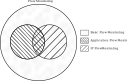
\includegraphics{figures/c03/flow-monitoring-types}
  \end{center}
  \caption{Relations between Different Flow Monitoring Types}
  \label{fig:flow-monitoring-types}
\end{figure}

% explain that application flow monitoring means that:
% - primary: information from application layer is added to flow records
% - secondary:
%  - application logic (not necessarily in L7) affect the flow creation process, e.g. monitoring of tunnels
%  - less typical but can also be considered as application flow monitoring: additional information can be added to flow records from external sources (geolocation)

We have already stated that application flow monitoring is a flow monitoring that uses application information. Let us now consider how that information can be used for creating flows and flow records. Firstly, the goal is to provide application layer information in the flow records. Therefore the flow record needs to be extended with fields containing information extracted from the application layer of the packets of the flow. Secondly, application logic can affect the flow creation process. For example, a flow with continuous HTTP connection can be split into multiple flows based on individual observed HTTP requests. Moreover, the application logic that affects flow creation is not be limited to application layer data, although the difference between basic flow monitoring and application flow monitoring is very thin in this case. Consider a scenario where Generic Routing Encapsulation (GRE) is used. As a basic flow, the GRE tunnel would be observed as a single flow. However, the GRE protocol can be considered an application, and by using the semantics of this application, we can split the single flow to many flows based on the traffic that flows through the GRE tunnel. Thirdly, additional information can be inserted from external sources based on the semantics of properties extracted from the packets. For example, geolocation information can be added to the flow records by the probe based on IP addresses of the communicating parties.

Now that the requirements for the application flow monitoring have been specified, we can formulate the application flow definition as follows:

\begin{definition}\label{def:application-flow}

    An \emph{\Index{application flow}} is a \emph{flow} where either
    the content of application layer or application logic is used
    to derive the flow keys.

\end{definition}

The definition specifies what an application flow is. Notice, however, that the definition does not cover all flows that are created by application flow monitoring. The problem is that the definition of application flow cannot specify how the subsequent flow record derived from the application flow will be created. For this reason, we need a definition of application flow record as well:

\begin{definition}\label{def:application-flow-record}

    An~\emph{\Index{application flow record}} is a \emph{flow record} 
    that contains information derived from either:

    \begin{enumerate}
        \item data contained in the application layer of the \emph{flow}, or
        \item external source of information.
    \end{enumerate}
        
\end{definition}

Application flow monitoring is a subset of flow monitoring where application flows or application flow records are used. Notice that application flow record can be created from standard flow record by extracting information from the application layer. Conversely, standard flow records can be created from application flows. Therefore, either the use of application flows or application flow records are enough to call the related monitoring process \emph{application flow monitoring}.

\section{Creating Application Flow}\label{sec:creating-application-flow}

Application flow monitoring significantly affects the whole flow monitoring process including the data processing on the collector. The most important impact is on the packet processing and flow creation processes of the flow exporter. The packet reception is not affected unless the packets are preprocessed in a hardware-accelerated NIC. This section describes important features of application flow monitoring and their impact on the flow monitoring process.

\subsection{Packet Processing}

The primary goal of packet processing is to extract values of chosen properties of individual packets and packet treatment information. Packet processing in basic flow monitoring can be done using simple packet parsers. These packet parsers only need to be able to process packet headers with simple structures, and the type of the following header is almost always determined by the content of the previous header. However, the type of application in the packet payload cannot usually be recognised from the packet headers. It is not necessary since every client must know where to connect and the server is expected to communicate only with clients using the correct protocol. Therefore, the flow exporters must identify the communicating applications themselves if they are to process the application payloads.

There are three techniques that are used for application identification nowadays. The first and oldest one is based on well-known port numbers assigned and maintained by IANA~\cite{IANA-2017-Service}. Although this method is very simple, fast, and easily implemented, it is not very precise. Since one of the goals of flow monitoring is to provide reliable data for network security, it would be easy for malicious parties to use ephemeral port numbers for their activities to hide their traffic. Moreover, well-known port numbers are often changed legitimately by administrators to improve security. Although this practice is condemned as a case of ``security through obscurity'', it helps to mitigate a large number of attacks. The second, more reliable, method of application identification is signature based. The application data of each protocol often carry a specific header which can be recognised by pattern matching. Such headers are usually present in the first packets of the connection; therefore the identification happens early enough for the packet processing to be able to process the relevant application data. There are several application identification libraries and related sets of signatures. The paper by \citeauthor{Bujlow-2015-classification}~\cite{Bujlow-2015-classification} compares the performance of two commercial and four open-source traffic classification tools. Thirdly, machine learning can be used for application identification, as described in Section~\ref{sec:app-rel-work}. However, these methods often require features that are available only after the flow is exported, such as the number of packets or timing between individual packets. Since machine learning cannot usually recognise the application after first data packet, which often contains the most important information, it is not used for traffic classification by flow exporters.

We have already shown examples of aggregated and non-aggregated basic flow properties in Chapter~\ref{chap:network-flow-monitoring}. Properties extracted from application data are mostly aggregated as they are not present in every packet of the flow. Moreover, they are very often present only in a single packet of the flow, e.g. the properties found in HTTP header or parameters of TLS connection during the handshake. The aggregation function applied in such cases is \emph{firstOf}, which means that the first value of the property is used. 

Basic flow records are usually created from the first layers of the packets. The most common example is flow monitoring skipping the \emph{link layer} (e.g. Ethernet), extracting information from the \emph{network layer} (e.g. IPv4 or IPv6) and the \emph{transport layer} (e.g. TCP, UDP, ICMP). However, the protocol encapsulation can be much more complicated. For example, protocols such as IP in IP, Generic Routing Encapsulation (GRE), and PPTP allow to create virtual connections and provide a second layer of headers in each packet. Basic flow monitoring usually creates flows from the first layer it encounters. However, when the flow exporter searches for application layer, it should traverse all underlying layers as well. Moreover, the layer from which the flow records are created must be well defined. It is even possible to create flows based on higher layers and therefore split a single basic flow record based on its content. More details on this process are provided in Chapter~\ref{chap:traffic-analysis-using-application-flow-monitoring}.

The creation of application layer parsers is a complicated process. Although there are several tools designed for this purpose, as shown in Section~\ref{sec:app-rel-work}, it is often more efficient to create a particular parser from scratch. We have built several application parsers by hand and using lexical analysis tools for the HTTP protocol and evaluated their performance in Section~\ref{sec:http-parser-design}.

\subsection{Flow Creation}

\begin{figure}[t!]
  \begin{center}
    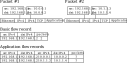
\includegraphics{figures/c03/encapsulation}
  \end{center}
  \caption{Traffic Encapsulation Example}
  \label{fig:encapsulation}
\end{figure}

The flow creation process is affected in two ways. Firstly, properties derived from application values can be part of a flow key. This is the case of encapsulated protocol where the payload contains more IP headers, as shown in the Figure~\ref{fig:encapsulation}. If the addresses of the second IP header are used in flow keys, the basic flow is split into multiple flows, as described in the previous section. Secondly, the flows can be split when a certain application event occurs. The description of the second case follows.

Application protocol measurement may require flow record to be expired early. For example, when HTTP protocol supports pipelining, multiple requests and responses can be carried out over a single connection. When it is desirable to keep track of each request/response pair, existing flow record might be exported when a new request is encountered on the same connection. This is an example of the situation in which application logic affects the creation of flows, for which reason they become application flows. Note that the application flow monitoring may affect the number of generated flow records. This needs to be taken into consideration during further processing of the flow records.

Based on the previous example, we can see that the application flow monitoring affects not only flow keys, but the flow expiration as well. Therefore, we add \emph{application event} to the existing flow expiration reasons (inactive timeout, active timeout, natural expiration, resource constraints, exporter termination). The application event expiration is usually implemented when the single connection is reused for multiple events of the same kind. Another example apart from the HTTP pipelining is FTP file transfer, where multiple files are transferred using a single connection, or SMTP connection where multiple messages are delivered at once.

The flow record values extracted from application layer are often present only in a single packet (e.g. HTTP header properties). This causes the information to be lost when the flow is long, and an active timeout is triggered. The new flow record cannot contain the application information since it is not present anymore during its creation. There are two ways to solve this issue. The first is to do nothing during the flow creation and handle the problem during flow data processing. The previous flow records can be looked up, and the necessary information can be extracted from them. The advantage of this method is that statistical queries about application layer data are not affected since the application data are always confined to a single record in this case. The second option is to copy the relevant application information to the new flow record upon active timeout. The information is then easily accessible during flow data processing; however, it is duplicated, and special care needs to be taken when performing statistical queries on the flow data. Either of these options can be taken, but the flow data processing system must be aware of it.

A negative impact of the application flow monitoring on the flow creation process is the increased size of flow records. The information extracted from application protocols can be quite large in comparison to network and transport layers lengths. While the typical IPv4 header length is 20 bytes, typical TCP header length is 32 bytes, and the HTTP URL can easily be several hundred bytes long. Therefore, the length of flow records of application flow monitoring is several times larger than without the application layer. There are two primary negative impacts of such large flow records. Firstly, the flow cache might require much more RAM than basic flow monitoring flow cache. Secondly, even if the cache fits into RAM, it degrades the performance of the memory accesses because data locality is decreased and a CPU experiences more cache misses. For these reasons, it must be carefully considered which information is placed in each flow record and how it is encoded.

\subsection{Flow Export}

The flow export is affected by application flow monitoring in two ways. Due to the larger flow records the amount of exported data increases. The second is that when a template based protocol such as IPFIX is used, the number of templates increases fast with each new combination of supported protocols.

The most important thing that changes for flow export when flow monitoring is applied is that the flow records might be much longer. This can cause congestion of the management link. When only a part of the data is necessary for flow processing on the collector, the exported data can be shortened. For example, only hostname and fixed length beginning of the URL can be exported for the HTTP protocol. However, since this leads to decreased quality of the exported data, information about the original data, such as original URL length, should be exported as well. The additional data allow the collector to correctly estimate the amount of missing information and apply the necessary algorithm to account for it. Long flow records also have a significant impact on flow record fragmentation when UDP protocol is used. Flow records longer than network interface MTU cannot fit into a single packet and must be fragmented, unless the transport protocol, such as TCP,  or flow export protocol handles fragmentation instead. The fragmentation puts additional load on flow collectors and causes increased data loss.

Exporters using template-based protocols, such as IPFIX, need to manage a significant number of templates when application flow monitoring is applied. This can cause performance issues since a template lookup needs to be performed for each flow record. Moreover, flow collectors need to process the templates as well. If the data are stored, for example, in a relational database and each template is represented by a table, a large number of tables can cause the queries to be slow since a union over many tables would need to be performed. Similar problems arise for other forms of flow storage and processing as well.


\section{Design of an HTTP Parser: A Study}\label{sec:http-parser-design}

It has been observed that the HTTP protocol became a ``new Transmission Control Protocol'' (TCP). More and more applications rely on HTTP protocol, e.g. Web 2.0 content, audio and video streaming, instant messaging, etc. HTTP traffic (TCP port 80) can usually pass through most firewalls and therefore presents a standard way of transporting/tunnelling data. The versatility, ubiquity, and amount of HTTP traffic make it easy for an attacker to hide malicious activities. Missing application layer visibility renders standard NetFlow and IPFIX to be ineffective for HTTP monitoring.

The research presented in this section attempts to answer the following question: What are the impacts of application layer analysis of HTTP protocol on flow exporters and flow monitoring process? The contribution of our work in this section is threefold: Firstly, we have designed and evaluated several HTTP protocol parsers representing current state-of-the-art approaches used in today's flow exporters. Secondly, we have introduced a new flex-based HTTP parser. Thirdly, we report on the throughput decrease (performance implications of application parser) which is of the utmost importance for high-speed deployments.

The rest of this section is organized as follows. Subsection~\ref{subsec:http-related_work} describes related work. Subsection~\ref{subsec:http-tool_design} contains a description of the HTTP inspection algorithms and the framework that was used to test the algorithms. Subsection~\ref{subsec:http-metodology} describes the methodology used for HTTP parsers performance comparison. Subsection~\ref{subsec:http-perform_evaluation} presents the performance evaluation of the individual algorithms. Finally, Subsection~\ref{subsec:http-conclusion} contains our conclusions.

\subsection{Related Work} \label{subsec:http-related_work}

Application layer protocol parsers are an integral part of many network monitoring tools. We explored the source code of the following frameworks to see how the HTTP parsing is implemented. nProbe uses standard glibc~\cite{GNUProject-2017-GNU} functions like \emph{strncmp} (compare two strings) and \emph{strstr} (locate a substring). YAF uses Perl Compatible Regular Expressions (PCRE)~\cite{Hazel-2015-PCRE} to examine HTTP traffic. Suricata~\cite{OISF-2017-Suricata} and Snort~\cite{Roesch-1999-Snort} are both written in C. Suricata uses LibHTP~\cite{Qualys-2017-LibHTP} library which does HTTP parsing using custom string functions while Snort does its parsing using glibc functions. httpry~\cite{Bittel-2014-httpry} is another HTTP logging and information retrieval tool which is also written in C and uses its own built-in string functions. These HTTP parsers are hand-written.

Another approach is taken by Bro~\cite{Paxson-1999-Bro} authors. They use binpac~\cite{Pang-2006-binpac}, which is a declarative language and its compiler designed to simplify the task of constructing robust and efficient semantic analysers for complex network protocols. They replaced some of Bro existing analysers (handcrafted in C++) and demonstrated that the generated parsers are as efficient as carefully hand-written ones.

In this section, we try to determine whether these approaches to HTTP parsing can handle large traffic volumes. Besides the above approaches, we propose to use the Fast Lexical Analyzer (Flex)~\cite{Levine-2009-Flex} to design a new HTTP parser. Flex converts expressions into a lexical analyser that is essentially a deterministic finite automaton that recognises any of the patterns. The algorithm that converts a regular expression directly to deterministic finite automaton is described in \cite{Lesk-1975-Lex} and \cite{McNaughton-1960-Regular}.

There are other works that inspect the HTTP protocol headers. In~\cite{Schneider-2008-new} the authors use statistical flow analysis to differentiate traditional HTTP traffic and Web 2.0 applications. In~\cite{Torres-2012-Identifying} the authors identify HTTP sessions based on flow information. In both cases, a ground truth sample is needed, which is a topic addressed by~\cite{Torres-2012-Strategies}. In~\cite{Gehlen-2012-Uncovering} and \cite{Mahanti-2011-Characterizing} the authors use DPI to obtain information from the HTTP headers. Our approach is orthogonal to these works since we are interested in extending basic flow records with HTTP data.

\subsection{Parser Design} \label{subsec:http-tool_design}

HTTP protocol~\cite{rfc7230} has a number of properties that can be monitored and exported together with basic flow data. The most commonly monitored ones are present in almost every HTTP request or response header. Based on the properties monitored by the state-of-the-art DPI tools we selected the following ones for our parsers: \emph{HTTP method, status code, host, request URI, content type, user agent and referer}. Keeping track of every bidirectional HTTP connection is too resource consuming on high-speed networks. Thus we focus on the evaluation of each individual packet. This approach is common for flow exporters since it is more resistant to resource depletion attacks.

% This should be floating, but it is impossible to get labels straight when wrapped in figure env.
\noindent\hspace{1pt}
\begin{minipage}[t]{(0.49\textwidth)-2pt}
\begin{algorithm}[H]
\caption{\emph{strcmp} }
\label{alg:strcmp}
{%\fontsize{8}{10}\selectfont
\begin{algorithmic}[1]
    \IF{first line contains ``HTTP''}
        \WHILE{\NOT end of HTTP header}
            \FOR{every parsed HTTP field}
                \IF{field matches the line}
                    \STATE{store the value of the line}
                \ENDIF
            \ENDFOR
            \STATE move to the next line
        \ENDWHILE
        \RETURN{HTTP packet}
    \ELSE 
        \RETURN{\NOT HTTP packet}
    \ENDIF
\end{algorithmic}
}
\end{algorithm}
\end{minipage}%
\hfill
\begin{minipage}[t]{0.47\textwidth}
\begin{algorithm}[H]
\caption{\emph{pcre}}
\label{alg:pcre}
{%\fontsize{8}{10}\selectfont
\begin{algorithmic}[1]
    \IF{first line contains ``HTTP/x.y''}
        \FORALL{PCRE rules}
            \IF{rule matches}
                \STATE{store the matched value}
            \ENDIF
        \ENDFOR
        \RETURN{HTTP packet}
    \ELSE 
        \RETURN{\NOT HTTP packet}
    \ENDIF
\end{algorithmic}
}
\end{algorithm}
\end{minipage}
\vspace{10pt}

We implemented and evaluated three different types of parsing algorithms. The first algorithm (\emph{strcmp} approach) loops the HTTP header line by line and searches each line for given fields. It uses standard glibc string functions like \emph{memchr}, \emph{memmem} and \emph{strncmp}. The simplified pseudocode is shown in Algorithm~\ref{alg:strcmp}. The second algorithm (\emph{pcre} approach) uses several regular expressions taken from YAF to search the packet for specific patterns indicating HTTP header fields. The pseudocode for the \emph{pcre} algorithm is shown in Algorithm~\ref{alg:pcre}. We designed the third algorithm (\emph{flex} approach) to handle each packet as a long string. It uses finite automaton to find required HTTP fields, and the Flex lexer is used to process the packets. The automaton design is shown in Fig.~\ref{fig:flex_schema}.

\begin{figure}[t]
        \centering
        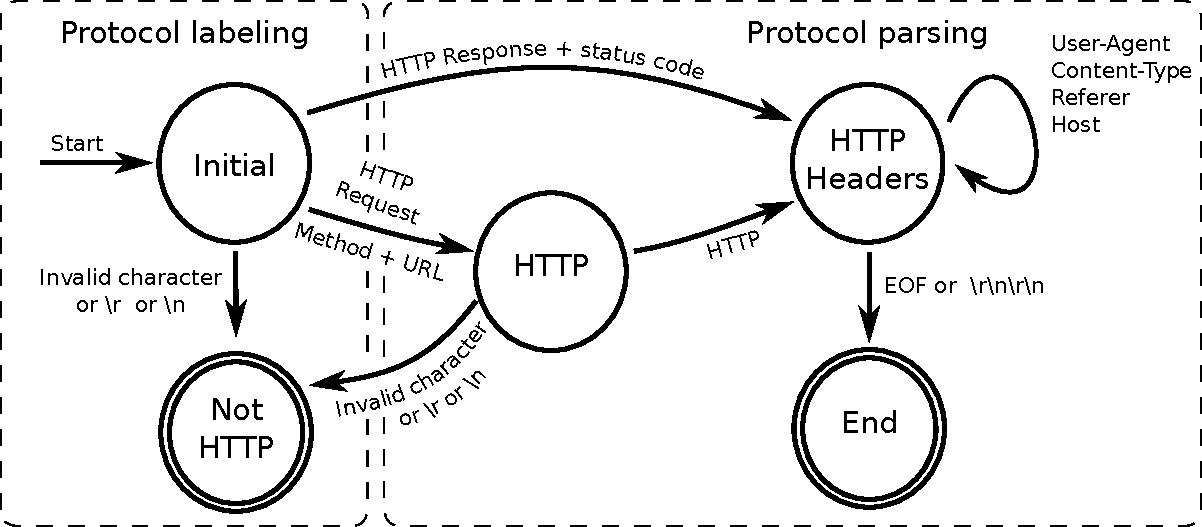
\includegraphics[width=0.8\textwidth]{figures/paper-http/flex_schema}
        \caption{\emph{flex} Algorithm Schema}
        \label{fig:flex_schema}
\end{figure}

Since the Flex is a generic tool, its initialisation before scanning each packet is quite an expensive operation. Therefore we decided to remove all unnecessary dynamic memory allocations and costly initialisations to see whether the performance can be increased. We named the new version \emph{optimized flex}. The disadvantage of Flex is that it has to keep the data in its own writeable buffer. Therefore the received data must be copied to such a buffer, which adds to the processing costs significantly. The advantage of the \emph{flex} parser is its simple maintenance and extension possibilities. The framework can be modified to parse any other application layer protocol just by changing the set of regular expression rules. The \emph{strcmp} parser would have to be rewritten from scratch.

The \emph{strcmp} implementation also offers a space for further improvement. Algorithm~\ref{alg:optimized-strcmp} shows an \emph{optimized strcmp} version of the code that features a better processing logic. The optimised version searches for specific strings by comparing several bytes at once, which is done by casting the character pointer to integer pointer. The number that is compared to the string is computed from ASCII codes of the characters and converted to network byte order. The size of the used integer depends on the length of the string; longer integers offer superior performance.

To focus only on the HTTP parsing algorithms, we decided to let the FlowMon exporter~\cite{FlowmonNetworks--Flowmon} handle the packet preprocessing. We used a  benchmarking (input) plugin that reads packets from PCAP file to memory at start-up. Then it supplies the same data continuously for further processing. This approach allows us to focus on benchmarking the algorithms without the necessity of considering the disk I/O operations. We provide the source code of implemented algorithms and used packet traces at our homepage~\cite{Sima-2013-FlowMon}.

\begin{algorithm}[tb]
\caption{\emph{Optimized strcmp}}
\label{alg:optimized-strcmp}
{%\fontsize{8}{10}\selectfont
\begin{algorithmic}[1]
    \IF{payload begins with ``HTTP''}
%       \STATE \COMMENT{HTTP response}
        \STATE store status code
        \WHILE{\NOT end of HTTP header}
            \FOR{every parsed response HTTP field}
                \IF{line starts with field name}
                    \STATE{store the value of the line}
                \ENDIF
            \ENDFOR
            \STATE move to the next line
        \ENDWHILE
        \RETURN{HTTP response packet}
    \ENDIF
    \IF{payload begins with one of GET, HEAD, POST, PUT,\\
            \hspace{\algorithmicindent}\hspace{\algorithmicindent}DELETE, TRACE, CONNECT}
%       \STATE \COMMENT{HTTP request}
        \STATE store request URI
        \WHILE{\NOT end of HTTP header}
            \FOR{every parsed request HTTP field}
                \IF{line starts with field name}
                    \STATE{store the value of the line}
                \ENDIF
            \ENDFOR
            \STATE move to the next line
        \ENDWHILE
        \RETURN{HTTP request packet}
    \ENDIF
    \RETURN{not HTTP packet}
\end{algorithmic}
}
\end{algorithm}

\subsection{Evaluation Methodology} \label{subsec:http-metodology}

In this section, we define a methodology of HTTP protocol parsers evaluation. We focus on parsing performance (number of processed packets per second) of the algorithms described in Section \ref{subsec:http-tool_design} from several different perspectives.

The first perspective focuses on the performance comparison with respect to analysed traffic structure. The second perspective covers the impact of the number of HTTP fields supported by the parser. The third perspective describes the effect of a Carriage Return (CR or \verb!'\r'!) and a Line Feed  (LF or \verb!'\n'!) control characters distribution in the packet payload.

A common technique of increasing network data processing performance is processing only important part of each packet. Therefore, we perform each of the tests in two configurations. In the first configuration, the parsers are given whole packets. This is achieved by setting the limit on packet size to 1500 bytes, which is the most common maximum transmission unit value on most Ethernet networks. In the second configuration, the parsers are provided with truncated packets of length 384 bytes, which is the minimum packet length recommended for DPI by authors of the YAF exporter~\cite{Inacio-2010-YAF}.

To test the performance of the parsers, we created an HTTP traffic trace (testing dataset). Our requirements on the dataset were as follows: preserve the characteristics of HTTP protocol, reflect various HTTP traffic structures and have no side effects on the flow exporter. In order to meet these requirements, we decided to create a synthetic trace.

The HTTP protocol is a request/response protocol. To preserve the characteristics of HTTP protocol during the testing a random request, response and binary payload packet were captured from the network. To omit the undesirable bias of the measurement only these three packets were used to synthesise test trace. The final test trace consists of 200 packets. In order to reflect various traffic structures, we suggested following ratio:

\begin{align}
       r = \frac{\# \text{request packets}+\#\text{response packets}}{\#\text{all packets}}*100
\end{align}

where $r \in [\,0,100\,]$ and created a test set for each integer ratio from the interval. Further, we created two packets with the modified payload. One packet contained the CR and LF control characters only at the very \emph{beginning} of the packet payload, the other one only at the \emph{end}. For both of the modified packets and the \emph{unchanged} packet, the test trace for each integer ratio was created.

% Network analysis tools trim the packets in order to increase throughput. However, we should set the trim limit to the smallest number that will capture the HTTP information we are interested in. We investigate the influence of the trim value on the performance; thus we select two limits. In the first case, we set the limit to 1500\,B which refers to the standard Ethernet frame length. In the other case, we set the limit to 384\,B which is recommended by YAF as a minimum payload length for the best results \cite{Inacio-2010-YAF}.

Having defined the test trace, we propose the following case studies to cover all evaluation perspectives. The case studies are carried out for both full and truncated packets. Moreover, we measure the performance of the flow exporter without an HTTP parser (\emph{no HTTP} parser). This way we can estimate the performance decline caused by increased application layer visibility.

\begin{enumerate}
    \item \emph{Performance Comparison}: This case study compares the parsing performance of implemented parsers. Moreover, we report on the flow exporter performance without an HTTP parser (\emph{no HTTP} parser).
    \item \emph{Parsed HTTP Fields Impact}: This case study shows a parser performance with respect to the number of supported HTTP fields. We incrementally add support for new HTTP fields and observe the impact on the parser performance.
    \item \emph{Packet Content Effect}: The result of this study presents the influence of the CR and LF control characters position in a packet payload on the parser performance. The test traces containing modified payload packets are used to perform the measurement.
\end{enumerate}

The performance evaluation process employs the benchmarking input plugin (see Subsection~\ref{subsec:http-tool_design}) to obtain the number of processed packets per second. 
In order to avoid influencing the results, the plugin uses a separate thread and CPU core for the accounting. The plugin counts the number of the processed packets in a ten-second interval and then computes the packets per second rate. We have operated the benchmark plugin for fifty seconds for each test trace and computed a number of packets processed and a standard error of the measurement. The parsed HTTP header fields impact and packet content effect were assessed in a similar way. All measurements were conducted on a server with the following configuration: Intel Xeon E5410 CPU at 2.33\,GHz, 12\,GB 667\,MHz DDR2 RAM and Linux kernel 2.6.32 (64 bit).

\subsection{Parser Evaluation} \label{subsec:http-perform_evaluation}

In this section, we present results of HTTP parser evaluation. First, we describe the parser performance comparison; then we investigate the impact of supported HTTP header fields. Finally, the effect of the packet content on HTTP parsing performance is shown.

\subsubsection*{Performance Comparison.}

This case study uses the standard version of each parser that supports seven HTTP fields. The dataset containing the unmodified payload packets is used, and the parsers are tested both on full and truncated packets. Fig.~\ref{fig:http-pcap_1500} shows the result for full packets case study and Fig.~\ref{fig:http-pcap_384} shows performance evaluation for truncated packets.

First we discuss the Fig.~\ref{fig:http-pcap_1500}. The \emph{no HTTP} meter is capable of parsing more than 11 million packets per second. This result is not influenced by the application data carried in the packet since the data is not accessed by the \emph{no HTTP} parser. Employing event the fastest of the HTTP parsing algorithms the performance drops to the nearly one-half of parsed packets per second. All of the HTTP parsers show the decrease in the performance as the ratio $r$ increases. This is caused by growing amount of request and response packets, which are more time demanding to parse.

\begin{figure}[tb]
        \centering
        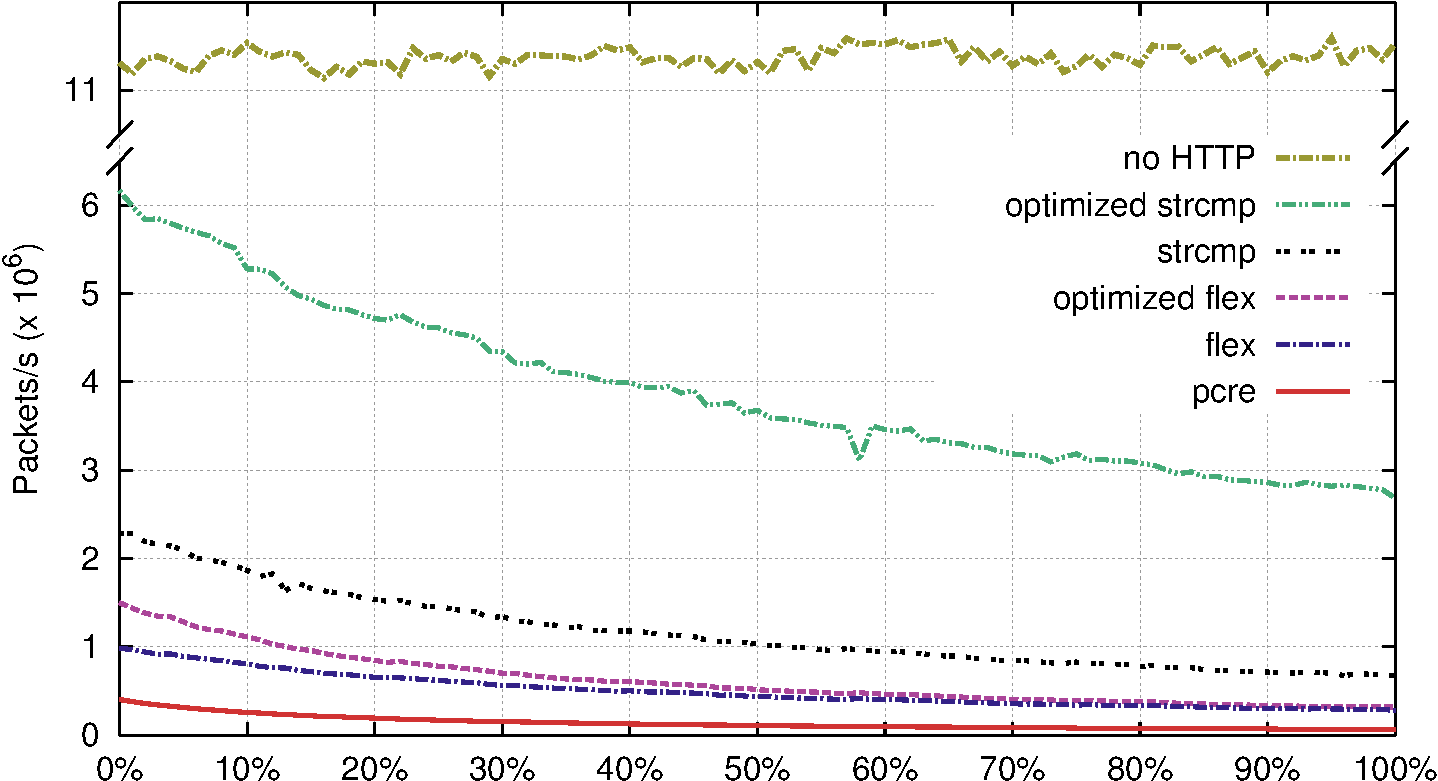
\includegraphics[width=0.8\textwidth]{figures/paper-http/1500_pcap_norm_1}
        \caption{Parser Performance Comparison with Respect to HTTP Proportion (0\,\% - No HTTP, 100\,\% - Only HTTP Headers) in the Traffic - Full Packets 1500\,B.}
        \label{fig:http-pcap_1500}
\end{figure}

The best performance is achieved by \emph{optimized strcmp} parser, which uses application protocol and code level optimisations. The parser takes into account the HTTP header structure, the difference between HTTP request and response headers and looks only for header fields that can be found in the specific header type. The code level optimisations include converting static strings into integers and matching them against several characters at once, which can be done in one processor instruction. The \emph{strcmp} parser performance is the second best, although the throughput is less than half of the \emph{optimized strcmp} parser.

The main difference between \emph{flex} and \emph{optimized flex} parsers is in the automaton initialization process. By rewriting the initialisation process, we achieved slight performance improvement, which is noticeable mainly in the $\langle\,0\,\%,20\,\%\,\rangle$ interval, where the actual HTTP parsing time is short. There is one other important factor affecting the \emph{flex} parser performance. The flex automaton is designed to work with its own writable buffer since it marks the end of individual parsed tokens directly into the buffer. For this reason, a copy of the packet payload must be created before the actual parsing can start. To measure the impact of the copying, we created another two parser plugins called \emph{empty} and \emph{copy}. First, we measured the flow exporter throughput with \emph{empty} plugin which performs no data parsing, then with \emph{copy} plugin which only copies packet payload to a static buffer. From the results, we estimate the throughput the \emph{optimized flex} parser would have without the memory copying. The performance of the \emph{optimized flex} parser would be about 2.4\,million packets per second for 0\,\% and 0.33\,million packets per second for 100\,\% HTTP packets. This shows that the actual HTTP parsing when compared to \emph{strcmp} parser, is slightly faster for binary payload packets and slower for HTTP header packets.

The performance of the \emph{pcre} parser is the lowest. The PCRE algorithm converts the regular expression to a tree structure and then performs a depth-first search while reading the input string. In case there is no match in the current tree branch, the algorithm backs up and tries another one. Therefore, for a complex regular expression, the pattern matching is not that fast as simple string search using functions like \emph{strcmp}. Another reason why the \emph{pcre} parser is not fast is that it performs all searches on whole packet payload. The other algorithms are processing the data sequentially.

\begin{figure}[tb]
        \centering
        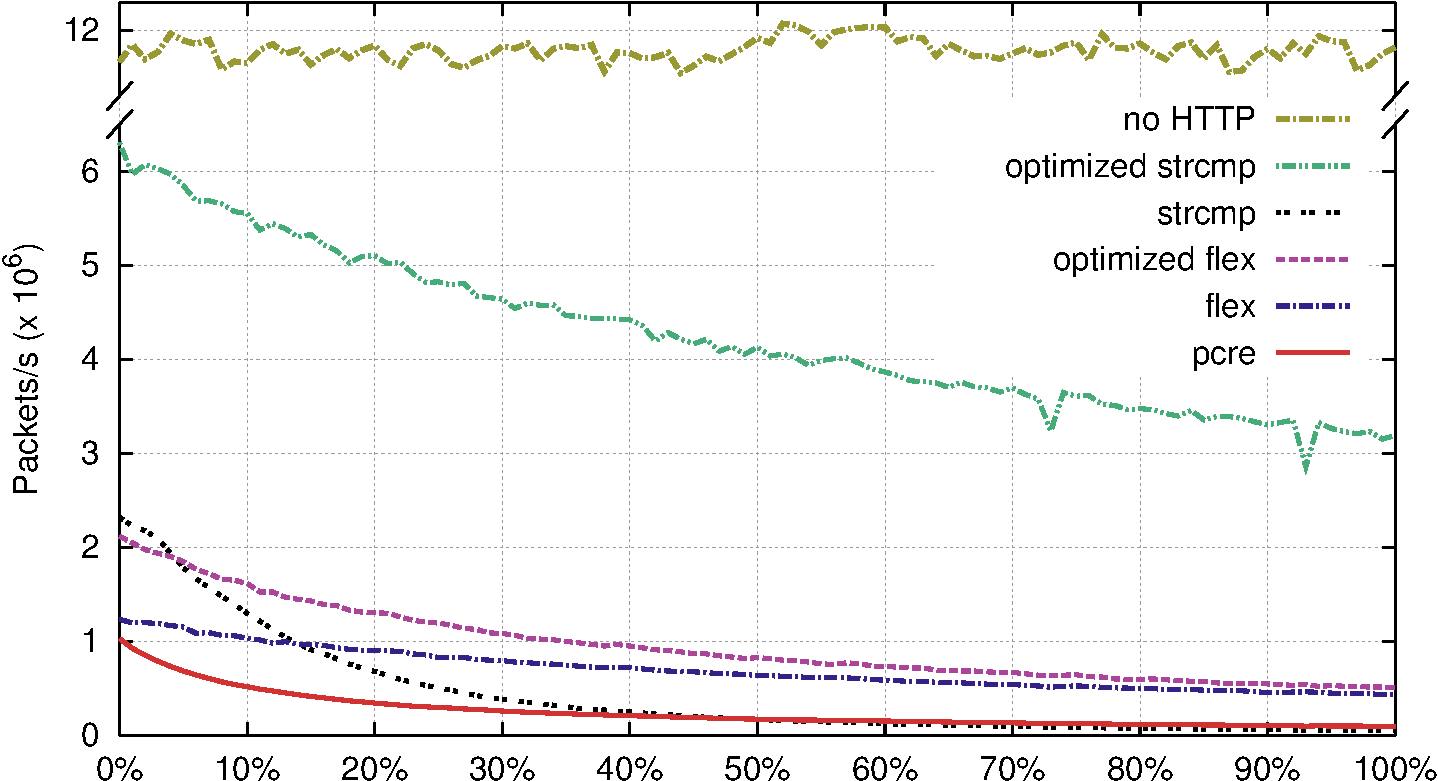
\includegraphics[width=0.8\textwidth]{figures/paper-http/384_pcap_norm_1}
        \caption{Parser Performance Comparison with Respect to HTTP Proportion (0\,\% - No HTTP, 100\,\% - Only HTTP Headers) in the Traffic - Truncated Packets 384\,B.}
        \label{fig:http-pcap_384}
\end{figure}

Fig.~\ref{fig:http-pcap_384} shows the results for truncated packets. The \emph{optimized strcmp} and \emph{no HTTP} are only slightly faster since the truncating of the packets has a positive impact on CPU data cache utilisation. The \emph{strcmp} algorithm is flawed since its throughput on HTTP packets deteriorates rapidly. This shows the disadvantage of hand-written parsers, as they are more error-prone than the generated ones. The \emph{pcre} parser performance is almost doubled, as the repeatedly processed data are truncated. Flex based parser also achieve performance increase, since the memory copying costs are reduced for smaller data.

\subsubsection*{Parsed HTTP Header Fields Impact.}

This case study was designed to show the impact of a number of parsed HTTP header fields on the parser performance. 

When payload packets are detected, they do not have their content parsed for additional HTTP header fields. Therefore, a test set containing only HTTP request and response packets was used. The case study starts with an empty plugin, that does not parse HTTP header fields and merely labels the HTTP packets. In the next steps, we cumulatively add further header fields to parse until we parse all of the seven supported fields. We run the tests for both full and truncated packets. The average performance of the parsers for each of the added field is shown in Fig.~\ref{fig:http-field}.

\begin{figure}[tb]
    \centering
    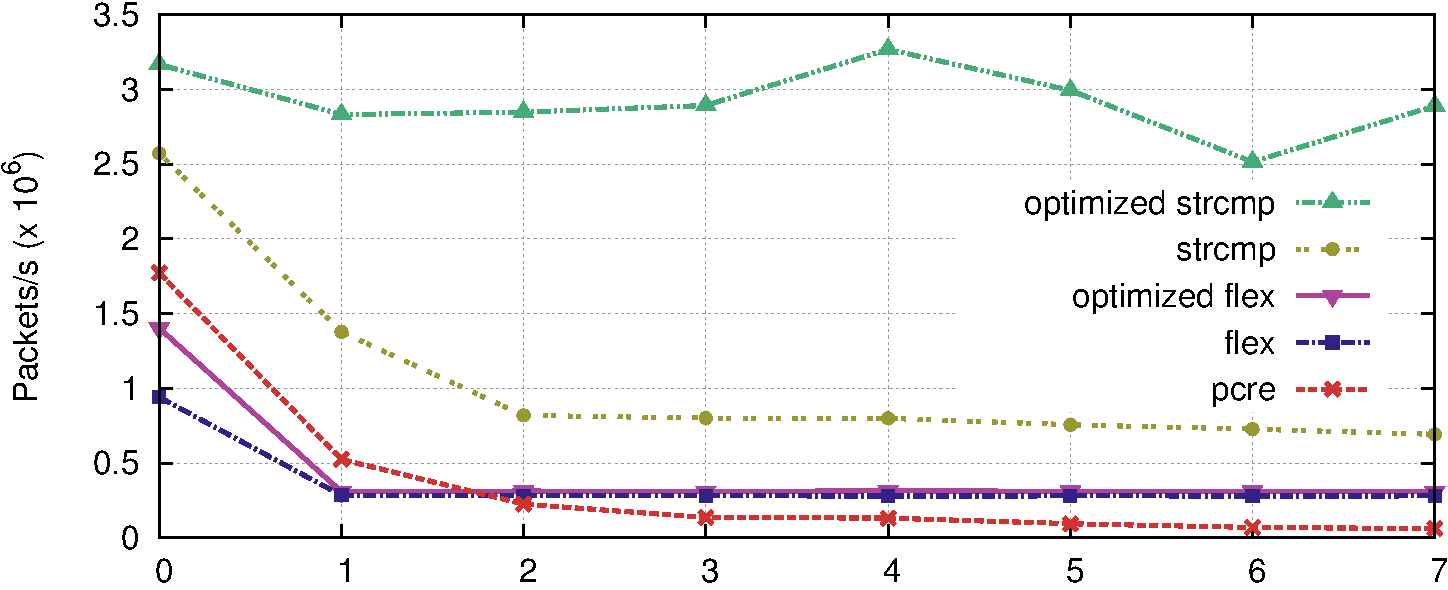
\includegraphics[width=0.8\textwidth]{figures/paper-http/mod_1500}
    \caption{An HTTP Parser Throughput for 1500\,B Packets; Supported Fields - (0) \emph{none} - HTTP Protocol labeling, (1) \emph{+host}, (2) \emph{+method}, (3) \emph{+status code}, (4) \emph{+request URI}, (5) \emph{+content type}, (6) \emph{+referer}, (7) \emph{+user agent}.} 
    \label{fig:http-field}
\end{figure}


Only the request and response packets are parsed, thus the values for the seven fields parsed in the Fig.~\ref{fig:http-field} correspond to the 100\,\% packet/s values in the Fig.~\ref{fig:http-pcap_1500} and Fig.~\ref{fig:http-pcap_384}. For the same reason the parsed packets per second numbers are lower in comparison with the Fig.~\ref{fig:http-pcap_1500} and Fig.~\ref{fig:http-pcap_384}. The performance of \emph{strcmp} and \emph{pcre} parsers drops with each additional parsed HTTP header field. The performance of the \emph{optimized strcmp} parser slightly fluctuates, as shown in Fig.~\ref{fig:http-field}. An example is the performance increase when adding a \emph{(4) request URI} or a \emph{(3) status code}. It is caused by extra code snippet that extracts the URI so that this line is not processed by the more generic code designed for parsing other header fields. Due to the usage of the finite automaton, the data is always processed in one pass by the flex-based algorithms. Therefore, they retain the same level of performance for all additional fields. This feature could be used to automatically build powerful parsers when a large number of parsed application fields would make it ineffective to create hand-written parsers.

Same as in the previous case study, the parsers processing truncated packets show better performance than the parsers working on full packets.

\subsubsection*{Packet Content Effect.}

This case study investigates the possible effects of the position of the CR and LF control characters in the packet payload on the parser performance. The mentioned ASCII characters represent the end of the line in the HTTP header. Some of the proposed algorithms use these characters as the trigger to stop parsing. Therefore the position of these characters affects the performance of the parsers. The packets with the CRLF characters at the very \emph{beginning} should be parsed faster than the packets having the CRLF at the \emph{end} since the algorithm terminates as soon as it identifies the CRLF characters. The test sets with modified binary payload packets (see Subsection~\ref{subsec:http-metodology}) enables us to compare the algorithms taking into account this perspective.

\begin{figure}[t]
    \centering
    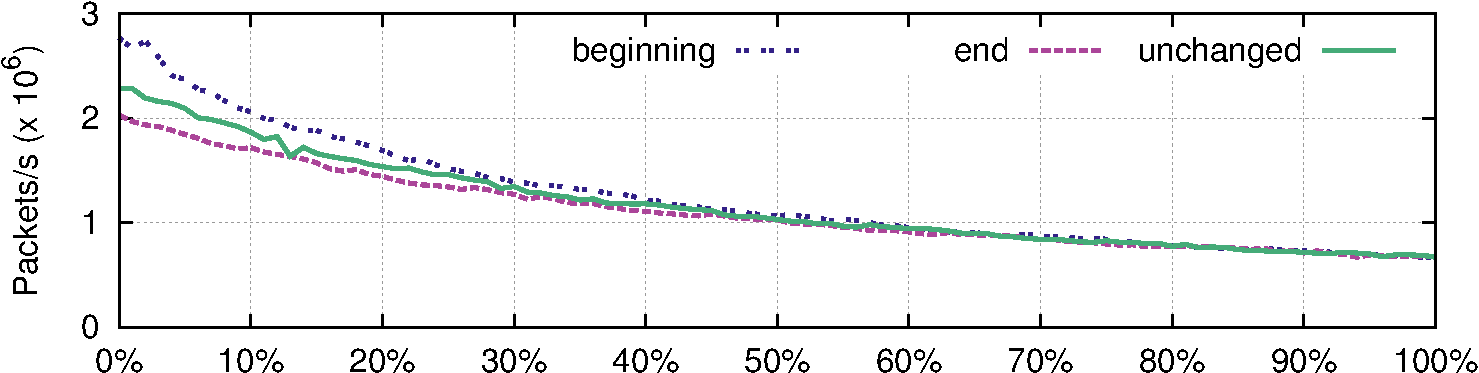
\includegraphics[width=0.8\textwidth]{figures/paper-http/1500_noflex}
    \caption{Packet Content Effect - Packet Length 1500\,B}
    \label{fig:http-packet_structure}
\end{figure}

We used the modified binary payload packets to test the parsers. The parsing algorithms, except the \emph{strcmp} algorithm, show an insignificant difference in their performance for all variants of the modified packets. The \emph{pcre} and \emph{optimized strcmp} parsers do not search for the end of line characters in order to label the packet; therefore this test does not affect them. The flex-based algorithms are not significantly affected since they stop parsing on the first character that is not expected in HTTP header and therefore stop at the first character in any case. The \emph{strcmp} parser depends on the search for end of line characters, which is confirmed by Fig.~\ref{fig:http-packet_structure}. The sooner the characters are found, the faster the algorithm terminates. The scenario with truncated packets is different since the performance on \emph{end} dataset is greater than on \emph{unchanged} data. This is caused by removing the end of packet payload together with the end of line character. When the \emph{strcmp} algorithm cannot find the character, it terminates immediately without trying to search the data. Therefore it terminates sooner than on an \emph{unchanged} dataset, where the end of line character is found, and the search continues.

\subsection{Conclusions} \label{subsec:http-conclusion}

This section has assessed the impacts of HTTP protocol analysis on flow monitoring performance. We implemented the state-of-the-art approaches to HTTP protocol parsing. Moreover, the new flex-based HTTP parser was designed, and its performance was compared to the other approaches.

The evaluation shows that in our case the hand-written and carefully optimised parser performs significantly better than implementations with automated parsing. It also shows that the new flex-based implementations handle the increasing number of parsed HTTP fields without significant performance loss. Truncating the packets prior to HTTP protocol parsing can increase the parser throughput. The performance comparison of \emph{no HTTP} parser with HTTP parsers shows that providing application visibility is a demanding task. Current approaches to the application protocol parsing may not be effective enough to process high-speed network traffic.

Although we focused on HTTP header parsing in this section, measuring the overall performance of flow exporters is also essential. We will address performance evaluation and runtime requirements of entire flow exporter frameworks in our future work. This research will allow us to compare existing frameworks and new prototypes under equal conditions. Monitoring of HTTP application protocol exposes new challenges for flow exporters. In particular, an increased number of exported fields, large flow record length and their impact on transport protocol requires further research.


\section{Summary}\label{sec:app-summary}

This chapter has described the aspects of extending flow monitoring by using information from the application layer. We have argued that application monitoring is necessary to provide information about current network-based cybersecurity threats. Without the application insight, attackers can perform application layer attacks that have no impact visible using the basic flow monitoring. Therefore the application flow monitoring utilises aspects of DPI to provide more fine-grained information about the observed traffic. 

We have briefly surveyed the state-of-the-art of the application parsers creation process. There are several approaches that allow creating application parsers from a higher level description, which allows creating more robust and error-prone parsers. However, existing application flow exporters do not often use these approaches and implement their own application parsers. Moreover, although most flow exporters support application identification, only a few of them provide real application visibility. 

The existing sources do not use consistent terminology regarding the application flow monitoring. Therefore, we have proposed a workable terminology that captures the current state of the art in the application flow monitoring. We call the flow monitoring without processing the application layer \emph{basic flow monitoring} and differentiate between \emph{IP flow monitoring} which is a term used for any flow monitoring that uses information from the IP layer. We have provided definitions of both \emph{application flow} and \emph{application flow record}, and explained their relation to the flow and flow record definitions provided in Chapter~\ref{chap:network-flow-monitoring}.

Once the terminology of application flow has been established, we ventured to describe the application flow monitoring process, particularly the changes that it introduced to the general flow monitoring process described in the previous chapter. It impacts the flow creation on two main levels. Firstly, a new flow expiration reason has been introduced that can be triggered due to an application event. Secondly, the flow records became application flow records as they contain information from the application layer. These changes have an impact on the number of generated flow records as well as on their sizes.

The last contribution of this chapter is a description of a design of an HTTP protocol parser. We have shown several approaches to the construction of the parser, implemented them and evaluated their performance. We have quantified the flow monitoring performance drop caused by each of them and showed, that a hand-crafted parser can be highly optimised to provide the best throughput, although it requires much more expert programmer to implement it correctly.

\chapter{Application Flow Monitoring Performance}

\iinfo{Text below is mostly from Challenges of Application Flow Monitoring.}

\itodo{FIX CITATIONS}

\itodo{TODO: Howto measure flow monitoring performance - skoro samostatná kapitola}
\itodo{TODO: biflow}
\itodo{TODO: Include more details}
\itodo{TODO: Give a background about high-speed packet capture, lucaderi, etc.}
\itodo{TODO: Put in papers from IM2015}
\itodo{TODO: Title is Flow Monitoring Performance, split to application and classic}
\itodo{Speedup by ommiting SSL/TLS processing for most application plugins}

\section{Accelerating Application Flow Monitoring}

We have shown that there are many different challenges when building application flow monitoring system. Most of the described processes are performance sensitive, especially packet reception, packet parsing, and flow aggregation. To achieve application flow monitoring throughput of tens of gigabits per second, several optimization and acceleration techniques can be applied. This section focuses on these techniques. Note that we avoid the use of sampling since it degrades the quality of exported data, as shown by the authors of~\cite{Brauckhoff-2006-Impact}. Although we describe acceleration techniques, their design, and main ideas, we will not go into details about their evaluation and testing, which is out of the scope of this article. 

It has been shown by the authors of~\cite{Velan-2015-High} that standard flow monitoring can achieve more than 100 Gb/s throughput on a commodity CPU when hardware accelerated NICs are used. The work of \citeauthor{Kekely-2016-Software}~\cite{Kekely-2016-Software} shows that it is possible to utilize these NICs to achieve 100 Gb/s throughput even for application flow monitoring. We discuss both hardware accelerated techniques and software optimizations in this section. Table~\ref{tab:flow-acc-techniques} gives an overview of the discussed techniques.


\begin{table}[ht!]
	\centering
	\begin{tabular}{|l|l|}
	\hline
	\textbf{Hardware acceleration} & \textbf{Software acceleration} \\ \hline
	Multiple reception buffers & Multithreading \\
	Packet trimming & NUMA awareness \\
	Packet header preprocessing & Flow state in parsers \\
	Flow processing offloading & Flow cache design \\
	Application identification & Flow cache timeouts \\ \hline
	\end{tabular}
	\caption{Flow Acceleration Techniques}
	\label{tab:flow-acc-techniques}
\end{table}


\subsection{Hardware Accelerated Techniques}

A field-programmable gate array (FPGA) is usually used in hardware accelerated network interface cards. It allows to parse packet headers and perform other tasks such as packet trimming or computing hashes to identify flows in the NICs. It usually supports transferring data to multiple buffers in RAM so that the software can efficiently use a multi-threading model. There are several manufacturers that provide such NICs, such as Napatech, Myricom, Mellanox Technologies, or Netcope Technologies. NICs can support hardware acceleration even without an FPGA chip, however, the capabilities are usually more limited and cannot be extended after the card is produced. For example, Intel produces many NICs without an FPGA chip that provide basic hardware acceleration such as packet hashing and transport to multiple RAM buffers.

By transferring data to multiple buffers in RAM, the NIC allows multiple CPU cores to process the data without any kind of locking mechanism. The data parsing is usually the most CPU intensive part of the application flow creation process, therefore it is very desirable to parallelize the computation. It is often necessary for the application packet parsing process to see multiple packets from the same flow. Therefore, it is desirable to store packets belonging to single flow to a single buffer in RAM, so that they are not processed by multiple different threads. To achieve this, the NIC must be able to correctly categorize packets belonging to the same flow. However, it is not necessary for the NIC to differentiate between every flow record. For example, when eight buffers are used, each flow must be sent to exactly one of the buffers. The easiest way to achieve this is to compute a three-bit hash from some of the flow-defining fields in the packet headers. IP addresses and transport layer ports are often used for this purpose, however, most manufacturers do not realize that this works incorrectly for fragmented packets. Therefore, it is better, in most scenarios, to use only IP addresses to distribute the flows to different buffers. The performance improvement achieved when using multiple buffers is directly related to the number of buffers. However, too many buffers introduce a high load on a memory controller causing the performance to be degraded. It is best to experiment with different numbers of buffers to find an optimal value for the target system. We have achieved the best results with 8-16 buffers, depending on the specific scenario and the number of CPU cores.

Memory throughput can easily become a bottleneck when data from 100\,Gb/s link are sent to RAM. One of the options to reduce the amount of processed data is to trim the received packets. Flow measurement without application protocols requires only packet headers up to the transport layer. Capturing the first 100 bytes of each packet is usually enough to contain various MPLS, VLAN, Ethernet, IPv6, and TCP headers. The rest of the packet can be discarded. The performance improvement achieved by this method depends on the average length of processed packets. However, application flow measurement requires also the packet payload. The amount of data that can be discarded varies depending on the measured application protocols. Unless the NIC has additional knowledge about measured traffic, it should not trim the packets at all for application flow measurement.

More radical way to save memory bandwidth and CPU cycles is to let the NIC extract the information required for flow monitoring and send only a special message with this information to the RAM. This process requires very specialized FPGA-based cards, such as COMBO series from CESNET. The performance gain can be quite high, as shown in~\cite{Velan-2015-High}. However, this method is not applicable for application flow measurement since application layer parsing is too complex and dynamic to be fully handled in the FPGA.

Packet trimming and packet parsing in the NIC are not usable for application flow monitoring. The main reason is that application layer parsing needs to be done in software. However, most packets do not carry application protocol headers. These packets can be processed by NIC and only extracted information transferred to software. Such a solution is proposed in~\cite{Kekely-2016-Software} and is called Software Defined Monitoring (SDM). It is based on offloading of heavy flows to the NIC. The important information from application layer is usually transferred in first N packets, where N can be expected to be lower than 20 in most cases. Therefore, after the software processing encounters the Nth packet, it instructs the NIC to process the rest of the flow. Only aggregated information about the flow is sent from NIC to software. The flow cache in the NIC is rather limited in comparison to the amount of RAM available in the software. However, only heavy flows need to be kept in this cache and it can be expired more often to reduce memory requirements. The authors show that 85 percent of traffic is observed in five percent of heavy flows. Therefore, the benefit of SDM has been shown to be an aggregation of 85 percent of packets to flow records in the NIC. This significant acceleration allows application flows to be monitored on 100\,Gb/s traffic. However, there is a downside to the SDM as well. Once a flow is offloaded to NIC, software parsers cannot observe further payloads containing subsequent application headers. For example, in the case of HTTP protocol the HTTP pipelining cannot be detected and information about further requests and responses in the same connection is lost.

Since only a small portion of all packets carry important application protocol information, it is beneficial to recognize such packets in the NIC and mark them for further processing in software. As the NIC cannot do complex application header processing, only a simple mechanism, such as pattern matching, can be utilized for packet classification. The work of the WAND Research Group~\cite{Alcock-2012-libprotoident} shows that it is possible to achieve reasonable traffic classification accuracy using only the beginning of a packet payload. Once the packets carrying application protocol headers are marked, the software parsers can process only these important packets. Moreover, other packets can be trimmed or parsed in the NIC and only important information can be passed for processing in the software. Packet classification can also benefit the SDM. When a flow is offloaded to NIC and a packet with application protocol header is matched, the processing of such a flow can be returned to the software. This approach would efficiently solve the abovementioned problem of HTTP pipelining. The accuracy and usability of pattern matching for packet classification depend on target application protocols and resource limitation of the NIC as well. Further research is needed to determine whether this method can be used for real world application flow monitoring.


\subsection{Acceleration in Software}

The performance of flow monitoring can be greatly enhanced by offloading as much of the necessary packet processing as possible to the NIC. However, to build a high-performance flow monitoring solution the software processing must be carefully tuned as well. Moreover, the FPGA-based NICs are much more expensive than commodity NICs and cannot always be deployed. This section focuses on flow monitoring optimizations that can be achieved by careful software design and system configuration.

The development of modern CPUs has a tendency to substitute raw power (frequency) by a higher number of CPU cores. To fully utilize the potential of a multi-core CPUs and achieve high flow monitoring performance, it is necessary to create multithreaded flow monitoring software. For NICs that support storing data in multiple buffers in RAM, the solution is to have different threads process the packets from different buffers. The resulting flow records are aggregated either in a single flow cache or in multiple flow caches, one per each thread, as shown in Figure~\ref{fig:exporter-thread-schema}. In either case, it must be ensured that there is a single thread used for exporting the resulting flow records where the data from multiple processing threads are merged. The latter approach is more effective as it clearly prevents the flow cache to become a point of contention. However, when there are multiple flow caches, it is necessary to ensure that each flow is aggregated in a single flow cache. This is ensured by having the NIC correctly distribute the packets to the buffers according to their association with their respective flow. Special care needs to be taken when the application protocol parsers need to process reverse flows as well. Both directions of the communication must be processed by the same thread. Using this approach, $N+2$ threads in case the first case or $2N+1$ threads in the second case can be utilized, where $N$ is the number of buffers and the last thread is used for flow export. 

\begin{figure}[t!]
  \begin{center}
    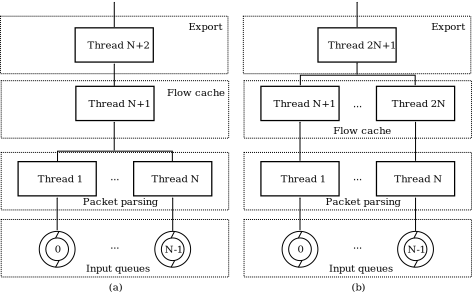
\includegraphics[width=\textwidth]{figures/exporter-thread-schema}
  \end{center}
  \caption{Multithreaded flow measurement with separate flow cache: a) single flow cache; b) multiple flow caches.}
  \label{fig:exporter-thread-schema}
\end{figure}

Separating packet parsing from flow cache management increases performance, however, processing application protocols may require a state of the connection to be kept. In such a case the flow cache record must be made available to the packet processing thread, which results in a use of synchronization primitives and overall performance decrease. One possible solution to this problem is to keep a different, smaller cache for chosen flow records directly in the packet processing thread. The only communication between the packet processing thread and the flow cache thread is a one-way passing of flow records, which can be done very effectively.

When a server with multiple CPUs is used, it is necessary to take care to assign each thread to correct CPU core. When the data is uploaded to RAM physically connected to different CPU than the packet processing core is running on, there is a performance hit for accessing the local memory of that CPU.

It is not effective to try every available application header parser on every packet to see which one is able to process it. When a packet from a flow was already matched by some application parser, it will usually not be matched by others. Therefore, by keeping the information about which flow is to be processed by each parser, most of the unnecessary and possibly expensive calls to application parsers can be eliminated. Moreover, when the flow is yet unmatched by any application parser, it is best to execute the application protocol parsers from the most common to the least common protocol.

One of the most performance critical parts of any flow measurement software is a flow cache. The cache needs to be designed to hold hundreds of thousands of flow records, do fast inserts, updates, and manage record expiration after active and inactive timeouts. It also needs to be robust and resilient enough to handle excessive workloads during DDoS attacks~\cite{Sadre-2012-Effects}. The flow cache design has been studied in the literature, for example in\cite{Wang-2011-Memory, Nassopulos-2014-Flow}. Although authors propose to use various data structures such as linked lists, trees, or multidimensional hashing table, our experience shows that the simplest solution is the best. The flow cache has to maintain data locality to make good use of CPU caches, therefore the dynamic structures do not perform as well as a simple hash table.

Flow cache inactive timeout expiration has a large impact on the performance, as shown in~\cite{Rodriguez-2013-Empirical, Molina-2006-Design}. The flow cache needs to be checked periodically to find and expire inactive records. However, doing the periodic checking in a separate thread requires extensive flow cache locking, which hinders the performance. Therefore, it is more efficient to dedicate part of the processing time of the flow cache thread itself to search for the inactive records. Carefully balancing the flow cache management tasks is a complex problem which offers a considerable potential for further research.

There are many other optimizations that can be performed to increase application flow monitoring performance, such as efficient flow key computation, processing packets in batches, ensuring CPU cache line alignment of flow records and so on. However, they are mostly a code micro-optimization no different from fine-tuning any other high-performance application and are out of the scope of this article.


\section{Conclusions}

\section{Relevant Publications}

\chapter{Measurement of Encrypted Traffic}

\section{Conclusions}

\section{Relevant Publications}


\chapter{Next Generation Flow}

\section{EventFlow}

\section{Flexible Flow Collector}

\itodo{
- IPFIXcol\\
- Collector design\\
- Problems with IPFIX protocol processing (Projít s Lukášem Hutákem)\\
- Flexible flow data storage (db vs nfdump vs FastBit vs new format?)\\

- Take a look at https://github.com/VerizonDigital/vflow
}

\section{Conclusions}

\section{Relevant Publications}

\itodo{
- AIMS 2012 ipfixcol design\\
- IM 2013 fbitdump vs nfdump comparison\\
- NOMS 2015 EventFlow
}

\chapter{Conclusions}

\section{Answers to Research Questions}

\section{Further Research}

%------------------------------------------------------------------------------

% Print bibliography at the end (should happen automatically,
% but this removes overleaf's warning)
\printbibliography[heading=bibintoc] %% Print the bibliography.

%------------------------------------------------------------------------------

% Print index
\makeatletter\thesis@blocks@clear\makeatother
\phantomsection %% Print the index and insert it into the
\addcontentsline{toc}{chapter}{\indexname} %% table of contents.
\printindex

%------------------------------------------------------------------------------

\appendix %% Start the appendices.
% List of authored publications

% Redefine fullcite to print all names, not just maxcitenames
\preto\fullcite{\AtNextCite{\defcounter{maxnames}{99}}}
\chapter{List of Authored Publications}

\section{Impacted Journals}

\begin{enumerate}
	\item \fullcite{my-Velan-2015-Survey}
\end{enumerate}

\section{Conference Proceedings}

\begin{enumerate}
  \item \fullcite{my-Hendriks-2017-Threats}
  \item \fullcite{my-Hendriks-2017-Flow}
  \item \fullcite{my-Velan-2016-Network}
  \item \fullcite{my-Velan-2016-EventFlow}
  \item \fullcite{my-Velan-2015-High}
  \item \fullcite{my-Pus-2015-Hardware}
  \item \fullcite{my-Husak-2015-Security}
  \item \fullcite{my-Velan-2014-Next}
  \item \fullcite{my-Velan-2013-Design}
  \item \fullcite{my-Velan-2013-Practical}
  \item \fullcite{my-Elich-2013-Investigation}
  \item \fullcite{my-Celeda-2013-Large}
  \item \fullcite{my-Velan-2012-Flow}
\end{enumerate}


\section{Other Publications}

\end{document}
